\documentclass[10pt]{article}


%% Packages
\usepackage{mathpazo}
%\usepackage{cmbright}
\usepackage{geometry}
\usepackage[numbers]{natbib}
\usepackage{amsmath}
\usepackage{amssymb}
\usepackage{amsthm}
\usepackage{amsfonts}
\usepackage{mathrsfs}
\usepackage{graphicx}
\usepackage{boxedminipage}
\usepackage{enumitem}
\usepackage{mathtools}
\usepackage{microtype}
\usepackage{setspace}
\usepackage{soul}
\usepackage{tikz}
\usetikzlibrary{arrows,fit,positioning,shapes,patterns,snakes,decorations,backgrounds}
\usepackage{algorithm}
\usepackage{algorithmic}
\usepackage{verbatim}
\usepackage{authblk}
\usepackage{extarrows}
\usepackage{titlesec}
\usepackage{color}
\usepackage{colortbl}
\usepackage{booktabs}
\usepackage{multirow}
\usepackage{hyperref}
\usepackage{centernot}

%% Colors
\definecolor{rred}{RGB}{204,0,0}
\definecolor{ggreen}{RGB}{0,145,0}
\definecolor{yyellow}{RGB}{255,185,0}
\definecolor{bblue}{rgb}{0.2,0.2,0.7}
\definecolor{ggray}{RGB}{190,190,190}
\definecolor{ppurple}{RGB}{160,32,240}
\definecolor{oorange}{RGB}{255,165,0}

%% Set margins and paper size
\geometry{verbose,letterpaper,tmargin=1in,bmargin=1in,lmargin=1in,rmargin=1in}
%% Nicer marginpar
\let\oldmarginpar\marginpar
\renewcommand\marginpar[1]{\-\oldmarginpar[\raggedleft\scriptsize\sf #1]{\raggedright\scriptsize\sf #1}}

%% Equation numbering
%\numberwithin{equation}{section}

%% Allow display breaks
\allowdisplaybreaks

%% Theorem-like environment settings
\theoremstyle{plain}
\newtheorem{theorem}{Theorem}
\newtheorem{lemma}{Lemma}
\newtheorem{proposition}{Proposition}
\newtheorem{corollary}{Corollary}

\theoremstyle{definition}
\newtheorem{definition}{Definition}
\newtheorem{assumption}{Assumption}
\newtheorem{conjecture}{Conjecture}
\newtheorem{example}{Example}

\theoremstyle{remark}
\newtheorem*{note}{Note}
\newtheorem*{claim}{Claim}

%% Define macros
\newcommand{\mb}{\mathbf}
\newcommand{\mcal}{\mathcal}
\newcommand{\tr}{^{\top}}
\newcommand{\subjectto}{\text{s.t.}}
\newcommand{\bA}{\mathbf{A}}
\newcommand{\bB}{\mathbf{B}}
\newcommand{\ba}{\mathbf{a}}
\newcommand{\bb}{\mathbf{b}}
\newcommand{\bd}{\mathbf{d}}
\newcommand{\bx}{\mathbf{x}}
\newcommand{\by}{\mathbf{y}}
\newcommand{\bu}{\mathbf{u}}
\newcommand{\bP}{\mathbf{P}}
\newcommand{\cP}{\mathcal{P}}
\newcommand{\cS}{\mcal{S}}
\newcommand{\OPV}{\text{OptVal}}
\newcommand{\T}{\mathcal{T}}
\newcommand{\Z}{\mathbb{Z}}
\newcommand{\R}{\mathbb{R}}
\newcommand{\notimplies}{\centernot\implies}


%% natbib settings
\bibpunct{[}{]}{;}{n}{}{,}

% Shrink section fonts
%\titleformat*{\section}{\normalsize\bf}
%\titleformat*{\subsection}{\normalsize\bf}
%\titleformat*{\subsubsection}{\normalsize\bf}


%% Double spacing
%\doublespacing

%% Paragraph spacing
\setlength{\parskip}{1ex}


%% ----- Begin document ----- %%
\begin{document}

%% Title of lecture, from class
\title{Research Meeting Notes}

%% Your name
\author{Jikai Zou}

%% Date
\date{Last updated: \today}

\maketitle

%%%%%%%%%%%%%%%%%%%%%%%%%%%%
\section*{April 14, 2014}
Currently we are working on the multi-stage stochastic generation expansion planning
problem and evaluating the performance of the approximation algorithm given by \cite{HA2009}.
Recall that the problem can be formulated as follows:
\begin{align*}
(\Pi_{\text{MS}}) \quad \min \quad & \sum_{n\in \T} p_n(\ba_n\tr \bx_n + \sum_{k\in K}\bb_{nk}\tr \by_{nk})\\
\subjectto \quad & \sum_{m\in\cP(n)} \bx_m \ge \bA_{nk}\by_{nk}, \quad \forall\; n\in \T, k\in K\\
& \sum_{m\in\cP(n)} \bx_m \le \bu, \quad \forall\; n \in S_T\\
& \bB_{nk}\by_{nk} = \mb{d}_{nk}, \quad \forall\; n\in \T, k\in K\\
& \bx_n\in \Z_+^{|I|}, \by_{nk}\in \R_+^{|J|}, \quad \forall\; n\in \T, k\in K.
\end{align*}
The approximation algorithm works as follows:
\begin{enumerate}
\item Solve the LP relaxation of $\Pi_{\text{MS}}$, obtain $(\bx^{LP},\by^{LP})$.
\item For each type of generator $i\in I$, solve
\begin{align*}
\min \quad & \sum_{n\in \T} p_na_{in}x_{in}\\
\subjectto \quad & \sum_{m\in\cP(n)} x_{im} \ge \lceil\bA_{nk}\by^{LP}_{nk}\rceil_i, \quad \forall\; n\in \T, k\in K\\
& \sum_{m\in\cP(n)} x_{im} \le u_i, \quad \forall\; n \in S_T\\
& \bx_n\in \R_+^{|I|}, \quad \forall\; n\in \T,
\end{align*}
and obtain $\{\bx_n^H, n\in \T\}$.
\item For each node $n\in \T$, solve
\begin{align*}
\min \quad & \sum_{k\in K}\bb_{nk}\tr \by_{nk}\\
\subjectto \quad & \sum_{m\in\cP(n)} \bx^{H}_m \ge \bA_{nk}\by_{nk}, \quad \forall\; n\in \T, k\in K\\
& \bB_{nk}\by_{nk} = \mb{d}_{nk}, \quad \forall\; n\in \T, k\in K\\
& \by_{nk}\in \R_+^{|J|}, \quad \forall\; n\in \T, k\in K.
\end{align*}
and obtain $\{\by_{nk}^H, n\in \T, k\in K\}$.
\item Return $\{(\bx_n^H, \by_{nk}^H), n\in \T, k\in K\}$.
\end{enumerate}

The following issues were addressed in today's meeting:
\begin{enumerate}[label=\emph{\alph*})]
\item {\bf If we implement this algorithm iteratively, will the solution keep improve and finally converge to the
optimal solution to the multi-stage problem?}
The answer is NO. For this problem, without considering lead time,
the algorithm ``always" stops at the second iteration (conclusion drawn
from numerical experiments, but not been proven yet.)
All numerical experiments show that $\by^H = \by^{LP}$.
Notice that though we have proven that $\sum_{m\in \cP(n)}{\bx^H_m} \ge  \sum_{m\in \cP(n)}{\bx^{LP}_m}$
for all $n\in \T$, and $\bA_{nk} \equiv \bA$ is a diagonal matrix $\text{Diag}(1/n_1^{max}, \dots, 1/n_{|I|}^{max})$,
this does not imply $\by^H = \by^{LP}$. It may happen that some component of $\by$ will increase
while others decrease, but together achieve a lower objective function value in the problem of Step 3.
Another thing noticed is that the operation cost obtained by solving problems in Step 3 seems always
equal to that in the LP relaxation (this is of course true if we can show that $\by^H = \by^{LP}$).

Things become a bit more complicated when we consider lead time in the model.
First, the answer to the raised question is still NO, i.e., the algorithm stops after
a certain number of iterations, same as the case without lead time. However, 
this number does not remain at 2 as before, I found instances that stop after the third
iteration. In addition, $\by^H$ is not the same as $\by^{LP}$ anymore. In particular,
the operations cost obtained by solving the problems in Step 3 seems smaller than
that in the LP relaxation. (What does this imply?)
One possible reason that $\by^H$ is not the same as $\by^{LP}$ anymore might be
existence of multiple optimal solutions. To see whether $\by^{LP}$ is better and $\by^H$
for the LP relaxation, we can fixed the $\by$ at $\by^H$ in the LP and solve for $\bx$,
and compare the optimal value with that of the original LP relaxation.
A possible related question is that what (if there is) does lead time change the structure of the problem,
in particular, the feasible regions?

\item Step 1 in the algorithm take quite a bit of time when planning horizon goes large.
{\bf Is there any decomposition method to solve the large scale LP?}

\item {\bf Think about the focus of the potential paper.}
One point is that we are solving the multi-stage problem instead of the two-stage problem.
What else? How do we interpret the ``hybrid" model?

\item {\bf Rolling horizon approximation.} This is still an open question. There are several ways
to approximate, e.g., solve exact two-stage problem in the rolling horizon fashion; 
use the heuristic to solve two-stage problem sequentially;
or approximate the multi-stage problem directly instead.
\end{enumerate}

%%%%%%%%%%%%%%%%%%%%%%%%%
\section*{April 21, 2014}
There are mainly two questions addressed during today's meeting:
\begin{enumerate}[label=\emph{\alph*})]
\item {\bf How to interpret/present the solutions of the multi-stage model and hybrid model?}
Notice that there is no uncertainty in the first period, and people only need the first several
decisions (w.r.t. periods) even if solving the problem of longer time horizon, we can compare
the solution of the first two periods in the two-stage and multi-stage models. Maybe we can
see how much flexibility the multi-stage model brings to us in terms of the expected cost.
Another way to examine the multi-stage solution is to look at the expected trajectory of the
solutions. This "expected" solution certainty may not be feasible, however, when compared
to the two-stage solution, it provides a reference of how conservative the two-stage solution is.
In terms of the hybrid model, we can test how fast the model converges to the multi-stage model
as the critical time $\tau$ increases, both in the sense of optimal value and solutions. 
\item {\bf How to translate a tree solution into a policy?}
Before addressing this question, we notice that solving the problem on ``a" specific scenario
tree does not buy us anything if the tree does not properly represent the underlying stochastic
process of the uncertain parameters. We know the optimal value will converge if we sample
enough from the tree, the question is how about the solution, or even the first stage solution?
Will the first period decision converges to the ground truth, i.e., the solution to the original
multi-stage stochastic problem, given the number of sample paths large enough?

Suppose solving the problem on a proper scenario tree gives ``valid" solutions, how can we
come up with a policy based on the solution? Two possible approaches were proposed:
\begin{itemize}
\item {\it``Find the closest scenario."}
Suppose we have solved the multi-stage problem on a given
scenario tree $\T$. Given a sample path $\xi^i = (\xi^i_1, \dots, \xi^i_T)$, we are about to find a decision
for $\xi^i$ based on the information we have, i.e., the optimal solution $x^*$ to the multi-stage problem on the
scenario tree. We do the following:
\begin{algorithm}
\caption{The Closest Scenario}
  \label{alg:cs}
  \begin{algorithmic}
    \FOR {$t = 1,\dots T$}
    \STATE $\omega^*_t \gets \arg \min\{d(\omega^k_t, \xi^i_t), k\in S_t\cap \T(\omega_{t-1}^*)\}$
    \STATE $x^i_t \gets x^*(\omega^*_t)$
    \ENDFOR
  \end{algorithmic}
\end{algorithm}
In the above policy, $d(\omega_1,\omega_2)$ is a pre-determined function that measures
the similarity of two parameter realizations $\omega_1$ and $\omega_2$, e.g., weighted average
of Euclidean distance of each uncertain parameter.
Therefore, we have a {\it static} policy as long as we have the solution to the tree problem.
%%%%%%%%%%%%%%%%
\item {\it``Rolling horizon approach."}
Given a sample path $\xi^i = (\xi^i_1, \dots, \xi^i_T)$, the first-stage decision $x^i$ for this
realization is obtained through the following procedure.
\begin{algorithm}
\caption{Rolling Horizon with Sampling}
  \label{alg:rh}
  \begin{algorithmic}
    \FOR {$t = 1,\dots T$}
    \STATE Generate a scenario tree $\T_t$ with root $\xi^i_t$ and length $T_0$
    \STATE Solve the multi-stage problem on $\T_t$ and obtain a optimal solution $\hat{x}^{(t)}$
    \STATE $x^i_t \gets \hat{x}^{(t)}_t$
    \ENDFOR
  \end{algorithmic}
\end{algorithm}
Notice that this provides us with a dynamic policy which is more adapted to the realization but
requires more computational effort. 
In the above procedure, one thing to point out is the choice of $T_0$,
it could be a fixed time period, e.g., $T_0 = T$ for every iteration;
it can also vary as we proceed, e.g., $T_0 = T-t$.
Note that we can apply this to the two-stage problem as well.
\end{itemize}
%%%%%%%%%%%%%%
\end{enumerate}
One thing to do immediately is to replicate the scenario tree generation method in \cite{J2011}.
Once we have a mechanism to generate scenario trees given the root information,
we can immediately implement two policies shown as above.

%%%%%%%%%%%%%%%%%%%%%%%%%
\section*{June 15, 2014: Policy Evaluation on A Deterministic Tree}
Suppose we are given a scenario tree, and we assume that this tree represents all possible
scenarios of the underlying stochastic processes associated with the uncertainty parameters.
The value of a given policy in such deterministic setting is considered as the total cost incurred
by implementing the policy on this deterministic scenario tree. In a two-stage policy, the first-stage
decision (corresponding to $\bx$ variables) is a static policy, i.e., it remains the same
for all scenarios in the tree. While in a multi-stage policy, the first-stage decision is adapted to
each possible outcomes at every time period.
However, the second-stage decision (corresponding to the $\by$ variables) is adapted to
each uncertainty realization in both two-stage and multi-stage policies.

Let us consider a multi-stage policy obtained by solving subproblems in the rolling horizon
framework. In particular, we consider the following deterministic version of Method \ref{alg:rh}:
\begin{algorithm}
\caption{Rolling horizon framework on a given scenario tree}
  \label{alg:rh_tree}
  \begin{algorithmic}
    \FOR {each node $n$ in $\T$}
    \STATE Solve a two-stage problem on the subtree $\T(n)$ and obtain a optimal solution
    $(\hat{\bx}^{(n)}, \hat{\by}^{(n)})$
    \STATE $(\bx^*_n, \by^*_n) \gets (\hat{\bx}^{(n)}_0,\hat{\by}^{(n)}_0)$
    // Fix the decisions at node $n$ with the root node decisions of the current subproblem
    \ENDFOR
    \RETURN $(\bx^*, \by^*)$
  \end{algorithmic}
\end{algorithm}


Note that in the first step of each for loop, if we solve a multi-stage subproblem instead of a
two-stage one, we again will obtain a multi-stage policy. It is clear that this policy is the same
as the one obtained by solving a large multi-stage problem on the whole tree $\T$, thus there
is no necessity of applying rolling horizon framework in such setting.

We now analyze the policy obtained in Method \ref{alg:rh_tree}.
It certainly is a feasible policy ({\color{rred}{not only the approximation problem on the tree,
but also the true problem?}}),
since the first-stage decision $\bx^*$ satisfies the upper bound
constraints and the second-stage problem is relatively completely recourse.

One can also specify the method used in solving each two-stage subproblem in each iteration.
If computation resource is not a restriction, we can solve the two-stage problem (MIP) exactly.
Alternatively, heuristics proposed in \cite{HA2009} can be applied to get an approximate solution.
{\color{rred}One interesting question is to investigate in how good this policy is, namely, how much is the
gap between the total cost of implementing such policy and that of implementing the optimal
multi-stage policy.}

\begin{table}[h]
\begin{center}
\scalebox{0.7}{
\begin{tabular}{cccccccccc}
\hline
\hline
& \multicolumn{9}{c}{\textbf{Time Horizon (T)}}\\
\textbf{Polices}                  & 2  	    & 3  	     & 4 	     & 5	      & 6  	      & 7 	       & 8 	         & 9  	    & 10 \\ \hline
\textbf{TS Heuristic}		  & 1713.80  &  3348.18 & 4642.37 & 7133.23 & 8687.73 & 10566.24 & 12507.59 & 14787.32 & 16249.05\\
\textbf{TS Optimal}             & 1713.80  & 3079.21 & 4598.61 & 6248.07 & 8054.33 & 9923.96 & 11870.43 & 13730.50 & 15660.19\\ 
\textbf{MS Heuristic}           & 1229.11  & 2357.96 & 3646.64 & 4991.92 & 6062.03 & 7433.84 & 8939.19  &  10341.38 & 11955.02\\
\textbf{MS Rolling Heuristic} & 1229.11 & 2357.96 & 3608.00 & 4865.01 & 5927.22 & 7302.31 & 8807.44  &  10251.53 & 11800.90\\ 
\textbf{TS Rolling Heuristic} & 1229.11 &  2376.82 &  3649.87 &  4850.81 &  5914.43 &  7343.69 &  8842.81 &  10261.58 & 11857.22\\ 
\textbf{TS Rolling Optimal}   & 1228.53 &  2148.61 &  3220.89 &  4441.54 &  5656.33 &  7026.48 &  8485.21 &  10013.92 & 11534.71\\
\textbf{MS Optimal}             & 1228.53 &  2138.57 &  3200.11 & [4321, 4355]  &  [5554, 5623] & [6914, 6990]  & [8344, 8505] & [9819, 10051] & [11303, 11971] \\ \hline \hline
\end{tabular}}
\end{center}
\vskip -0.4cm
\caption{Total costs incurred by different policies (unit: million dollars)}
\label{tb1:policy_test_deterministic}
\end{table}

\begin{figure}[h!]
\begin{center}
\includegraphics[scale=0.4]{figs/rolling_horizon_deterministic.eps}
\end{center}
\vskip -0.5cm
\caption{Total costs incurred by different policies}
\label{f1:policy_test_deterministic}
\end{figure}

\begin{figure}[h!]
\begin{center}
\includegraphics[scale=0.6]{figs/TS_optimal.eps}
\end{center}
\vskip -0.5cm
\caption{Optimal capacity planning of two-stage model}
\label{f2:TS_optimal}
\end{figure}


Numerical results are shown in Table \ref{tb1:policy_test_deterministic}  and Figure \ref{f1:policy_test_deterministic}.
Optimal capacity planning schedule for the two-stage model is shown in Figure \ref{f2:TS_optimal}.
For a given generation capacity planning problem with time horizon $T$, we evaluate four types
of policies:
\begin{enumerate}[label=\emph{\roman*)}]
\item \textbf{TS Optimal}: optimal static two-stage policy;
\item \textbf{MS Heuristic}: multi-stage policy obtained by heuristic in \cite{HA2009};
\item \textbf{TS Rolling Heuristic}: multi-stage policy obtained in the rolling horizon framework by solving each two-stage subproblem heuristically;
\item \textbf{TS Rolling Optimal}: multi-stage policy obtained in the rolling horizon framework by solving each two-stage subproblem exactly;
\item \textbf{MS Optimal}: optimal multi-stage policy.
\end{enumerate}

We have the following observations:
\begin{enumerate}[label=\emph{\alph*)}]
\item With the current problem parameters, the performance of these policies follows the sequence:
{\color{rred}TS Heuristic $\prec$ TS Optimal $\prec$ MS Heuristic $\sim$ TS Rolling Heuristic $\prec$ TS Rolling Optimal $\prec$ MS Optimal}.
Here the sign $A \prec B$ means Policy B is preferred to (dominated by) Policy A,
and the sign $A \sim B$ indicates that Policies A, B are not dominated by each other.
\item In general, the following preference are clear:
\begin{itemize}
\item {\color{rred}TS Heuristic $\prec$ TS Optimal $\prec$ TS Rolling Optimal $\prec$ MS Optimal};
\item {\color{ggreen}TS Heuristic $\prec$ TS Rolling Heuristic $\prec$ TS Rolling Optimal $\prec$ MS Optimal};
\item {\color{bblue}MS Heuristic $\prec$ MS Optimal}.
\end{itemize}
\item The following pairs of relationships are interesting to know:
\begin{itemize}
\item {\color{rred}TS Rolling Optimal v.s. MS Heuristic.}
In the current problem setting, TS Rolling Optimal outperforms MS Heuristic in all problems with time
horizon from $2$ to $10$. However, this is not true in general, consider the following setting.
We consider a two-period planning problem with one type of generator. The only uncertainty is demand.
At period 1, the demand is 10, and the demand at the second period is 20 with probability $0.4$, and 7 with probability $0.6$.
It costs 5 units of money to built one generator at the first period and 10 units in the second period.
We assume that there is no operating cost and no discount is considered here.
In addition, the capacity of the generator is 1 and all demand has to be satisfied.
Therefore, the multi-stage problem can be formulated as follows:
\begin{align*}
\min \quad & 5x_1 + 4x_2 + 6x_3\\
\text{s.t.} \quad & x_1 \ge y_1, x_1+x_2 \ge y_2, x_1 + x_3 \ge y_3\\
& y_1 \ge 10, y_2 \ge 20, y_3 \ge 7\\
& x_1, x_2, x_3\in \Z_+, y_1, y_2, y_3 \in \R_+
\end{align*}
The heuristic solution is the same as the optimal solution, i.e., (10, 10, 0).
On the other hand, TS Rolling Optimal in this instance is (20, 0, 0). Clearly, MS Heuristic $\succ$ TS Rolling Optimal.
A good explanation of this instance is that the initial demand is not zero and the cost of building one generator
is not monotone decreasing as $t$ increases, thus, in the optimal two-stage solution, everything will be build at the
beginning. However, since the cost is multiplied by the probability in later periods in the multi-stage model, some node
can have smaller building cost than previous period, hence some generator will be hold to build in the later period.
\item {\color{rred}TS Rolling Heuristic v.s. TS Optimal.}
It seems clear that TS Rolling Heuristic should be better than TS Optimal, since the former one is a multi-stage
policy after all. In the above example, TS Rolling Heuristic gives $(20, 0, 0)$, while TS Optimal yields $(20, 0)$,
TS Optimal is as good as TS Rolling Heuristic.
\emph{It would be good if there is an instance where TS Optimal performs
better than TS Rolling Heuristic.}
\end{itemize}
\item The main task here is to find out the gap between TS Rolling Optimal (Heuristic) and MS Optimal.
{\color{rred}In particular, we would like to have a upper/lower bound for cost(TS Rolling Optimal) - cost(MS Optimal).}
A possible intermediate step is to find out the gap between TS Rolling Optimal and TS Optimal.
First, note that TS Rolling Optimal can be as bad as TS Heuristic/TS Optimal (see the above example).
\end{enumerate}

\section*{July 24, 2014}
\begin{itemize}[itemsep=0ex,topsep=0ex]
\item Complete the computational result table
\item Set the time limit, optimality gap and other parameters to a reasonable value
\item Draw conclusions from the table
\end{itemize}

%%%%%%%%%%%%%%%%%%%%%%%%%%%%
\section*{September 14th, 2014}
Things finished last week:
\begin{itemize}[itemsep=0ex,topsep=0ex]
\item Second version of draft finished last week
\item Reviewed a first paper during the weekend
\end{itemize}

Regarding the current version of paper, there are several possible extension to the current model:
\begin{enumerate}[label=\emph{\roman*)}, topsep=0ex, itemsep=0ex]
\item In the current model, we have not considered the entire power grid, i.e., the current
generation expansion planning problem is solved by ``a" generator company.
We can also consider a centralized expansion planning problem where generators are build
across different sites, thus constraints on transmission line need to be taken into account.
\item For the decentralized generation expansion planning model, transmission constraints
can also be considered.
Recall the original model
\begin{subequations}
\begin{align}
\min \quad & \sum_{n\in \T}\left(\sum_{i\in \mcal{I}}\frac{p_nc_im_i^{max}}{(1+r)^{t_n-1}}x_{in}
	+ \sum_{i\in \mcal{I}}\sum_{k\in \mcal{K}_{t_n}}\frac{p_nh_kb_{ink}}{(1+r)^{t_n-1}}v_{ink} 
	+ \sum_{k\in \mcal{K}_{t_n}}\frac{p_nh_k q}{(1+r)^{t_n-1}}w_{nk}\right)\label{ge:obj}\\
\text{s.t.} \quad & \sum_{m\in \cP(n)}x_{im} \ge \frac{1}{n_i^{max}}v_{ink},
\quad \forall\; i\in \mcal{I}, n\in \T, k\in \mcal{K}_{t_n}\label{ge:capacity}\\
& \sum_{m\in \cP(n)}x_{in} \le u_i^{max}, \quad \forall\; i\in \mcal{I}, n\in \cS_T\label{ge:ub}\\
& \sum_{i\in \mcal{I}}v_{ink} + w_{nk} = d_{nk}, \quad \forall\; n\in \T, k\in \mcal{K}_{t_n}\label{ge:demand}\\
& x_{in_1} = x_{in_2}, \quad \forall\; i\in \mcal{I}, m\in \mcal{S}_{\eta}, n_1, n_2\in \T(m)\cap \mcal{S}_t,t>\eta\label{ge:na}\\
& x_{in}\in \Z_+, v_{ink}, w_{nk}\in \R_+, \quad \forall\; i\in \mcal{I}, n\in \T, k\in \mcal{K}_{t_n}.\label{ge:variable}
\end{align}
\end{subequations}
The above model does not consider where the generators are built or the transmission line
load between these sites. Now let's consider the set $\mcal{U}$, where contains all possible
construction site. Let $\mcal{L}$ be the set of transmission lines.

Then the extended model now becomes 
\begin{subequations}
\begin{align}
\min \quad & \sum_{n\in \T}\left(\sum_{i\in \mcal{I}}\sum_{u\in \mcal{U}}\frac{p_nc_im_i^{max}}{(1+r)^{t_n-1}}x_{i,u,n}
	+\sum_{i\in \mcal{I}} \sum_{u\in \mcal{U}}\sum_{k\in \mcal{K}_{t_n}}\frac{p_nh_kb_{ink}}{(1+r)^{t_n-1}}v_{i,u,n,k} 
	+ \sum_{k\in \mcal{K}_{t_n}}\frac{p_nh_k q}{(1+r)^{t_n-1}}w_{n,k}\right)\label{ge2:obj}\\
\text{s.t.} \quad & \sum_{m\in \cP(n)}x_{i,u,m} \ge \frac{1}{n_i^{max}}v_{i,u,n,k},
\quad \forall\; i\in \mcal{I}, u\in \mcal{U}, n\in \T, k\in \mcal{K}_{t_n}\label{ge2:capacity}\\
& \sum_{u\in \mcal{U}}\sum_{m\in \cP(n)}x_{i,u,n} \le u_i^{max}, \quad \forall\; i\in \mcal{I}, n\in \cS_T\label{ge2:ub}\\
& x_{i,u,n_1} = x_{i,u,n_2}, \quad \forall\; i\in \mcal{I}, u\in \mcal{U}, m\in \mcal{S}_{\eta}, n_1, n_2\in \T(m)\cap \mcal{S}_t,t>\eta\label{ge2:na}\\
& \sum_{i\in \mcal{I}} \sum_{u\in \mcal{U}}v_{i,u,n,k} + w_{n,k} = \sum_{u\in \mcal{U}}d_{u,n,k}, \quad \forall\; n\in \T, k\in \mcal{K}_{t_n}\label{ge2:demand}\\
& f_{\ell,n,k}^{min} \le \sum_{i\in \mcal{I}}\sum_{u\in \mcal{U}}\sigma_{u,\ell}v_{i,u,n,k} - \sum_{u\in \mcal{U}}\sigma_{u,\ell}d_{u,n,k} \le f_{\ell,n,k}^{max},
\quad \forall\; \ell\in \mcal{L}, n\in \T, k\in \mcal{K}_{t_n}\label{ge2:transmission}\\
& x_{i,u,n}\in \Z_+, v_{i,u,n,k}, w_{n,k}\in \R_+, \quad \forall\; i\in \mcal{I}, u\in \mcal{U}, n\in \T, k\in \mcal{K}_{t_n}.\label{ge2:variable}
\end{align}
\end{subequations}
%
We write this as a generic model
%
\begin{subequations}
\begin{align}
\min \quad & \sum_{n\in \T}p_n\left(\sum_{u\in \mcal{U}}\ba_{u,n}\bx_{u,n} +\sum_{u\in \mcal{U}}\bb_{u,n}\mb{v}_{u,n} 
	+ \mb{c}_n \mb{w}_n\right)\label{hb2:obj}\\
\text{s.t.} \quad & \sum_{m\in \cP(n)}\bx_{u,m} \ge \bA_{n,k}\mb{v}_{u,n},
\quad \forall\; u\in \mcal{U}, n\in \T, k\in \mcal{K}_{t_n}\label{hb2:capacity}\\
& \sum_{u\in \mcal{U}}\sum_{m\in \cP(n)}\bx_{u,n} \le \mb{u}^{max}, \quad \forall\; n\in \cS_T\label{hb2:ub}\\
& \bx_{u,n_1} = \bx_{u,n_2}, \quad \forall\; u\in \mcal{U}, m\in \mcal{S}_{\eta}, n_1, n_2\in \T(m)\cap \mcal{S}_t,t>\eta\label{hb2:na}\\
& \bB_{n}\sum_{u\in \mcal{U}}\mb{v}_{u,n} + \mb{I_{\mcal{K}_{t_n}}}\mb{w}_{n} = \sum_{u\in \mcal{U}}\bd_{u,n}, \quad \forall\; n\in \T\label{hb2:demand}\\
& \mb{f}_{\ell,n}^{min} \le \sum_{u\in \mcal{U}}\sigma_{u,\ell}\left(\mb{\Lambda_{n}}\mb{v}_{u,n} - \bd_{u,n}\right) \le \mb{f}_{\ell,n}^{max},
\quad \forall\; \ell\in \mcal{L}, n\in \T\label{hb2:transmission}\\
& \bx_{u,n}\in \Z_+^{I}, \mb{v}_{u,n}\in \R_+^{J_n}, \mb{w}_{n}\in \R_+^{K_n}, \quad \forall\; u\in \mcal{U}, n\in \T,\label{hb2:variable}
\end{align}
where $I = |\mcal{I}|$, $J_n = |\mcal{I}||\mcal{K}_{t_n}|$, and $K_n = |\mcal{K}_{t_n}|$.
\end{subequations}
%
Notice that model \eqref{hb2:obj} - \eqref{hb2:variable} is also decomposable in a way as before.
In order to prove that this extended model can still be solved by the heuristics in \cite{HA2009},
it remains to show that the coefficient matrix for constraints \eqref{hb2:capacity} - \eqref{hb2:na}
is TU. Let us investigate if this is true in the multi-stage model, i.e., $\eta=T$.

We have known that the coefficient matrix corresponding to constraint \eqref{hb2:capacity} is TU,
let $M$ be the corresponding LHS matrix. We want to show that
\[\tilde{M} = \left[\begin{array}{cccc}M & 0 & 0 & 0 \\0 & M & 0 & 0 \\0 & 0 & \ddots & 0 \\0 & 0 & 0 & M \\M & M & \cdots & M\end{array}\right]\]
is also TU.
\begin{conjecture}
If $M$ is TU, then $\tilde{M}$ is TU.
\end{conjecture}
It turns out the above conjecture is not correct. Here is one counter-example:
\begin{example}
When $M$ is from a 3-period 2-regular tree, $[M,0; 0,M; M,M]$ is indeed TU. But the three-bus case $[M,0,0; 0,M,0; 0,0,M; M,M,M]$ is not a TU.
Indeed, for a general TU matrix $M$, $[M,0; 0,M; M,M]$ is not necessarily TU.
For example, $M=[1,0,0,1;1,1,0,0; 0,1,1,0; 0,0,1,1; 1,1,1,1]$ is TU and not from a tree,
but the above block matrix with two $M$ is not TU. 
\end{example}

Therefore, with this formulation of transmission constraints, it is not clear how to apply the same analysis.
\end{enumerate}

%%%%%%%%%%%%%%%%%%%
\section*{September 17, 2014}
The analysis for lower bound on between two-stage and hybrid model, namely $v^{TS} - v^{HB}$,
remains almost the same as in the current draft, the only thing we need to change is in the beginning,
we use an LP solution $y$ from the two-stage model instead of the hybrid model.
Then we can obtain bounds for hybrid model with single generator in the same form,
but with those delta's defined w.r.t. the the previous mentioned $y$. Everything else follows.

However, both these bounds are not very interesting in our case.
In fact, they are negative in every instance. I think I said there were some
positive numbers for smaller instances in my previous testing,
unfortunately, I forgot to subtract the sum of investment cost in the first period.
Adding that part makes all of them negative...very very negative...

The main reason is that there is no uncertainty in the investment cost of generators,
and discount factor is also considered in our problem.
This results in a decreasing factor $(1+R)^{-1}$ in investment cost across time periods.
Even if we use smaller discount factor (extreme case: no discount), this still doesn't help much.
The reason for which is that demands are not very large, and recall those "delta"'s roughly equal
how many generators we need to cover the demand, in the LP solution, some of the generators are
just not needed. Putting this back to the expression in (3.18)(see the current draft),
the value is simply negative.

Noticed that in \cite{HA2009}, they present a lower bound of relative value of multi-stage stochastic programming,
which is a $(v^{ts}_{LP} - v^{ms}_{HEUR}) / v^{ts}_{LP}$, I calculated those numbers with
better upper bound (from MIP solver) on $v^{ms}$, and these numbers make sense.
But I still haven't been able to argue why somebody should choose hybrid model over multi-stage model.

Next to do: take a look at the policy generated by different models maybe something interesting there.

%%%%%%%%%%%%%%%%%%%%%%%%%%%%%%
\section*{September 20, 2014}

Since the investment costs are decreasing across time period due to the discount factor,
which looks like one can optimize the multi-stage problem by solving the problem \emph{only} for period 1
and record the investment decision. Then move to period 2 and solve the problem \emph{only} for period 2
conditioning on that he has built some number of generators (recorded) in period 1.
So on and so forth, he would solve the multi-stage problem by expanding capacities optimally just for the current period.

However, after solving the entire problem by periods, the solution is not the same as the multi-stage optimal solution.
The intuition is that in the true optimal solution, one would rather over build some capacities (e.g., build a nuclear power plant)
in early period even though that period's demand can be covered by building two other types of generators (e.g., CC) at a lower cost.
The fact is that in later periods, he has to build a nuclear generator to cover the higher demands later,
so solving this problem by period could result in expanding capacities in a inefficient way.

An interesting phenomenon is that:
{\color{rred}under the assumption that the investment cost is the same over periods,
solving the problem with $\mu=2$ in the rolling horizon framework
and recording the root solution can recover the multi-stage optimal solution.}
Applying this method and the results shows that the investment decision and total cost obtained are both
the same as the optimal multi-stage solution and cost for problem $T=3 \text { and } 4$.
Since we couldn't solve those larger multi-stage problems to optimality, we can only compare the total cost.
The result shows that such ``heuristic" achieves a smaller cost than the current best upper bound on the cost
when we solve the entire MIP.

Let us first examine the case where there is no operation decisions $y$.
In particular, we would like to address the following question:
\begin{quote}
Given that the investment costs remains the same across time period and discount factor
is considered, will the above heuristic recover the multi-stage optimal solution?
\end{quote}

Without the operation decisions, the multi-stage model can be written as
\begin{align*}
\min \quad & \sum_{n\in \T} p_n\ba_n\tr \bx_n\\
\subjectto \quad & \sum_{m\in\cP(n)} \bx_m \ge \bd_n, \quad \forall\; n\in \T\\
%& \sum_{m\in\cP(n)} \bx_m \le \bu, \quad \forall\; n \in S_T\\
& \bx_n\in \Z_+^{|I|}, \quad \forall\; n\in \T,
\end{align*}
where $\ba_n = \ba(1+\delta)^{-t_n}$. Notice that this problem is decomposable w.r.t.
different types of generators, we only need to consider the problem with one type of generators.
Since the LHS matrix is TU, we can assume $d$ and $u$ are integers and relax the integrality constraints.
Let us first look at the structure of the optimal multi-stage solution $x^*$.
\begin{claim}
For all $n \in \T$, $x^*_n = (d_n - \sum_{m\in \cP(a(n))}{x^*_m})_+$.
\end{claim}
\begin{proof}
Clearly, $x^*_n \ge (d_n - \sum_{m\in \cP(a(n))}{x^*_m})_+$.
Now assume that there exists $n_0$ such that $x^*_{n_0} > (d_{n_0} - \sum_{m\in \cP(a(n_0))}{x^*_m})_+$.
Let $\Delta = x^*_{n_0} - (d_{n_0} - \sum_{m\in \cP(a(n_0))}{x^*_m})_+>0$.
If $n_0\in S_{T}$, then decreasing $x^*_{n_0}$ by $\Delta$ results in a feasible but strictly better solution, contradiction.
Otherwise, decrease $x^*_{n_0}$ by $\Delta$, and increase $x^*_{n}$ by $\Delta$ for each $n\in C(n_0)$.
This solution is still feasible but decreases the total cost by $p_{n_0}a\Delta((1+\delta)^{-t_{n_0}} - (1+\delta)^{-t_{n_0}-1})>0$,
contradiction to the optimality of $x^*$.
We can apply this argument on every node $n$ with $x^*_{n} > (d_n - \sum_{m\in \cP(a(n))}{x^*_m})_+$,
then it follows that $x^*$ has the desired structure.
\end{proof}

Now let us examine the structure of the solution obtained by applying the above heuristic, we call this solution $\hat{\bx}$.
We show that $\hat{x}_n = x^*_n$ for all $n\in T$ by induction.
There is only one node in $S_1$, namely the root node. If $\hat{x}_1 > d_1$, reduce $\hat{x}_1$ to $d_1$ and increase
$\hat{x}_n$ by $\hat{x}_1-d_1$ for all $n\in S_2$. The new solution remains feasible but achieves a lower cost, contradiction.
Suppose for all $n\in S_t$, $t\le s\le T-1$, we have $\hat{x}_n = x^*_n$.
We next show that $\hat{x}_n = x^*_n$ for all $n\in S_{s+1}$.
Indeed for all $n\in S_{s+1}$ we have $x_n\ge (d_n - \sum_{m\in \cP(a(n))}\hat{x}_m)_+$,
and $x_n$ is the root solution of the current problem.
Since $a_{s+1}>a_{s+2}$, optimal solution $\hat{x}_n$ must be equal to $(d_n - \sum_{m\in \cP(a(n))}\hat{x}_m)_+$.
Thus we have proven that $\hat{x}_n = x^*_n$ for all $n\in T$.

However, the real question we want to address here is whether this property will change
if operation decisions are considered in the model.


\section*{September 24, 2014}\label{092414}
Using the same heuristic without considering the integrality constraints of investment decisions,
we observe differences between the optimal multi-stage cost and heuristic cost, even for instance
with $T=4$. However, when we do not allow penalty and set generation cost of each type of
generators to be the same,
it can be shown that {\bf the heuristic solution is indeed optimal}.
Under such setting, the multi-stage model becomes
\begin{align*}
\min \quad & \sum_{n\in \T}\sum_{i\in \mcal{I}}p_n(a_{in}x_{in} + b_{n}y_{in})\\
\subjectto \quad & \sum_{m\in \cP(n)}x_{im} \ge k_iy_{in},\quad \forall n\in \T, i\in \mcal{I}\\
& \sum_{m\in \cP(n)}x_{im} \le u_i, \quad \forall n\in \mcal{S}_T, i\in \mcal{I}\\
& \sum_{i\in \mcal{I}}y_{in} = d_n, \quad \forall n\in \T\\
& x_{in}, y_{in}\ge 0, \quad \forall n\in \T, i\in \mcal{I}.
\end{align*}
Notice that the objective function in above model is equivalent to
\[\min \quad \sum_{n\in \T}p_n\sum_{i\in \mcal{I}}a_{in}x_{in} + \sum_{n\in \T}p_nb_{n}d_n.\]
Let $(\hat{\bx}, \hat{\by})$ be the heuristic solution.
Thus $(\hat{\bx}_1, \hat{\by}_1)$ is the first component of an optimal solution
of the following problem
\begin{align*}
\min \quad & \sum_{n\in \T}p_n\sum_{i\in \mcal{I}}a_{in}x_{in} + \sum_{n\in \T}p_nb_{n}d_n\\
\subjectto \quad & \sum_{m\in \cP(n)}x_{im} \ge k_iy_{in},\quad \forall n\in \T, i\in \mcal{I}\\
& \sum_{m\in \cP(n)}x_{im} \le u_i, \quad \forall n\in \mcal{S}_T, i\in \mcal{I}\\
& \sum_{i\in \mcal{I}}y_{in} = d_n, \quad \forall n\in \T\\
& x_{in_1} = x_{in_2}, \quad \forall n_1,n_2\in \mcal{S}_t\cap \T(n), t\ge 3, n\in \mcal{S}_2\\
& x_{in}, y_{in}\ge 0, \quad \forall n\in \T, i\in \mcal{I}.
\end{align*}
Since the generation cost does not effect the preference of generators,
and the investment cost of each type of generators is decreasing across time
period, it is not hard to use a similar argument as above to show that one
will not over build capacities in each period. The question left is which generator
will be used in the optimal solution. I claim that at each node, the generator
with the lowest $a_{in}k_i$ value will be used until the demand at that node is covered
or the cumulated $x$ value along the path to node $n$ reaches $u_i$,
if in the latter case, the generators with the second lowest $a_{in}k_i$ value will be used,
so and so forth. (Note that without loss of generality, we can assume generators have
different $a_{in}k_i$ values.)
To see this, we can let $\bar{x}_{in} = \frac{x_{in}}{k_i}$ for all $n\in \T, i\in \mcal{I}$.
Hybrid problem is equivalent to 
\begin{align*}
\min \quad & \sum_{n\in \T}p_n\sum_{i\in \mcal{I}}a_{in}k_i\bar{x}_{in} + \sum_{n\in \T}p_nb_{n}d_n\\
\subjectto \quad & \sum_{m\in \cP(n)}\bar{x}_{im} \ge y_{in},\quad \forall n\in \T, i\in \mcal{I}\\
& \sum_{m\in \cP(n)}\bar{x}_{im} \le \frac{u_i}{k_i}, \quad \forall n\in \mcal{S}_T, i\in \mcal{I}\\
& \sum_{i\in \mcal{I}}y_{in} = d_n, \quad \forall n\in \T\\
& \bar{x}_{in_1} = \bar{x}_{in_2}, \quad \forall n_1,n_2\in \mcal{S}_t\cap \T(n), t\ge 3, n\in \mcal{S}_2\\
& \bar{x}_{in}, y_{in}\ge 0, \quad \forall n\in \T, i\in \mcal{I}.
\end{align*}
Then it is obvious that the above claim is correct. Otherwise we can move amount of
generation from a generator with higher $a_{in}k_i$ value to the one with the lowest
$a_{in}k_i$ value, still satisfying demand but achieving a lower cost.

Similar argument can be applied directly to the multi-stage model, which results in the
a same investment decision as the one obtained by heuristic.
Therefore, the heuristic LP-policy is indeed optimal.

Now let us look at a problem closer to the original problem: no penalty is allowed.
\begin{align*}
\min \quad & \sum_{n\in \T}\sum_{i\in \mcal{I}}p_n(a_{in}x_{in} + b_{in}y_{in})\\
\subjectto \quad & \sum_{m\in \cP(n)}x_{im} \ge k_iy_{in},\quad \forall n\in \T, i\in \mcal{I}\\
& \sum_{m\in \cP(n)}x_{im} \le u_i, \quad \forall n\in \mcal{S}_T, i\in \mcal{I}\\
& \sum_{i\in \mcal{I}}y_{in} = d_n, \quad \forall n\in \T\\
& x_{in}\in \Z_+, y_{in}\in \R_+, \quad \forall n\in \T, i\in \mcal{I}.
\end{align*}
%
It is equivalent to show that
\begin{quote}\bf
Given the number of available generators,
solving the multi-stage model and the hybrid model (with $\mu=2$) result in the same
first period solution.
\end{quote}

\section*{September 26, 2014}
TOO BAD...... The argument that I tried to show is not correct.
This is observed through the testing cases. In particular, I solved a 5-year planning problem
using this heuristic, and pass the obtained investment solution to the original multi-stage problem,
and solve it starting from this solution.
Indeed, better feasible solution is found. I terminate the solver once a better feasible
solution shows up, then find the nodes where the investment decisions are different.
Notice that some of the nodes are leaves or roots of a 2-period subtree, it is easy to calculate
the optimal solutions on these small subtrees.
The results show that in the current feasible solution, the solution corresponding to
these subtrees are not even optimal. This further shows that the heuristic solution is not optimal.
In particular, the following Gurobi log demonstrate what stated above.
\vskip 0.5cm
\begin{minipage}[t]{4.2cm}
\tiny\begin{verbatim}
4354.86573107 3181.65484134 1173.21088973

4354.70693981 3179.62437697 1175.08256284

35
[1, 0, 0, 0, 0, 0]
[0, 0, 0, 0, 0, 2]
93
[1, 0, 1, 0, 0, 0]
[0, 2, 2, 0, 0, 0]

n 35 g 0 t 0
1130.0 0.0
n 35 g 0 t 1
1130.0 0.0
n 35 g 0 t 2
564.200913242 0.0
n 35 g 1 t 1
125.461187215 135.461187215
n 35 g 2 t 0
324.746575342 334.746575342
n 35 g 5 t 0
560.0 1680.0
\end{verbatim}
\end{minipage}
\begin{minipage}[t]{4.2cm}
\tiny\begin{verbatim}
n 35 g 5 t 1
560.0 1680.0
n 35 g 5 t 2
560.0 1124.20091324
n 93 g 0 t 0
2260.0 1130.0
n 93 g 0 t 1
2260.0 1130.0
n 93 g 0 t 2
1409.31506849 1130.0
n 93 g 1 t 0
780.0 1560.0
n 93 g 1 t 1
94.1095890411 1224.10958904
n 93 g 1 t 2
0.0 279.315068493
n 93 g 2 t 0
652.568493151 1002.56849315
n 106 g 0 t 0
1130.0 0.0
n 106 g 0 t 1
928.02739726 0.0
n 106 g 0 t 2
312.328767123 0.0
\end{verbatim}
\end{minipage}
\begin{minipage}[t]{4.2cm}
\tiny\begin{verbatim}
n 106 g 1 t 0
670.267123288 680.267123288
n 106 g 5 t 0
560.0 1680.0
n 106 g 5 t 1
560.0 1488.02739726
n 106 g 5 t 2
560.0 872.328767123
n 107 g 0 t 0
1130.0 0.0
n 107 g 0 t 1
1130.0 0.0
n 107 g 0 t 2
1130.0 0.0
n 107 g 1 t 1
1141.36073059 1151.36073059
n 107 g 1 t 2
215.662100457 225.662100457
n 107 g 2 t 0
1282.76712329 1292.76712329
n 107 g 5 t 0
560.0 1680.0
n 107 g 5 t 1
560.0 1680.0
\end{verbatim}
\end{minipage}
\begin{minipage}[t]{4.2cm}
\tiny\begin{verbatim}
n 107 g 5 t 2
560.0 1680.0
n 108 g 0 t 0
1130.0 0.0
n 108 g 0 t 1
1130.0 0.0
n 108 g 0 t 2
1130.0 0.0
n 108 g 1 t 2
251.643835616 261.643835616
n 108 g 2 t 0
1344.83561644 1354.83561644
n 108 g 2 t 1
18.1369863014 28.1369863013
n 108 g 5 t 0
560.0 1680.0
n 108 g 5 t 1
560.0 1680.0
n 108 g 5 t 2
560.0 1680.0
[[[102, 0], 0.5479452054942158]]
[[[102, 0], 0.547945205463293]]
\end{verbatim}
\end{minipage}

\begin{minipage}[t]{8cm}
\tiny\begin{verbatim}
####################################################################################
Loaded MIP start with objective 5296.89

Variable types: 72 continuous, 20 integer (0 binary)

Root relaxation: objective 5.186323e+03, 60 iterations, 0.00 seconds

    Nodes    |    Current Node    |     Objective Bounds      |     Work
 Expl Unexpl |  Obj  Depth IntInf | Incumbent    BestBd   Gap | It/Node Time

     0     0 5186.32264    0    7 5296.89180 5186.32264  2.09%     -    0s
     0     0 5214.99087    0    4 5296.89180 5214.99087  1.55%     -    0s
     0     0 5220.40982    0    3 5296.89180 5220.40982  1.44%     -    0s
     0     0 5220.40982    0    7 5296.89180 5220.40982  1.44%     -    0s
     0     0 5220.40982    0    3 5296.89180 5220.40982  1.44%     -    0s
     0     0 5229.97790    0    5 5296.89180 5229.97790  1.26%     -    0s
     0     0 5229.97790    0    5 5296.89180 5229.97790  1.26%     -    0s
H   11     0                    5281.1433720 5235.64046  0.86%   1.4    0s
*   12     0              11    5280.8351252 5235.64046  0.86%   1.7    0s

Cutting planes:
  Gomory: 6

Explored 71 nodes (238 simplex iterations) in 0.02 seconds
Thread count was 4 (of 4 available processors)

Optimal solution found (tolerance 1.00e-04)
Best objective 5.280835125216e+03, best bound 5.280835125216e+03, gap 0.0%
5280.83512522 [[1, 0, 0, 0, 0, 0], [0, 0, 0, 0, 0, 0], [0, 1, 3, 0, 0, 0], [0, 1, 3, 0, 0, 0]]

####################################################################################
\end{verbatim}
\end{minipage}
\begin{minipage}[t]{8cm}
\tiny\begin{verbatim}
####################################################################################
Loaded MIP start with objective 3981.56

Variable types: 18 continuous, 5 integer (0 binary)

Root relaxation: objective 3.782530e+03, 14 iterations, 0.00 seconds

    Nodes    |    Current Node    |     Objective Bounds      |     Work
 Expl Unexpl |  Obj  Depth IntInf | Incumbent    BestBd   Gap | It/Node Time

     0     0 3782.53047    0    2 3981.55863 3782.53047  5.00%     -    0s
     0     0 3810.90898    0    3 3981.55863 3810.90898  4.29%     -    0s
     0     0 3855.96117    0    2 3981.55863 3855.96117  3.15%     -    0s
     0     0 3876.92878    0    1 3981.55863 3876.92878  2.63%     -    0s
     0     0 3876.92878    0    1 3981.55863 3876.92878  2.63%     -    0s
H    1     0                    3944.0309363 3876.92878  1.70%   0.0    0s

Cutting planes:
  Gomory: 3

Explored 19 nodes (54 simplex iterations) in 0.01 seconds
Thread count was 4 (of 4 available processors)

Optimal solution found (tolerance 1.00e-04)
Best objective 3.944030936253e+03, best bound 3.944030936252e+03, gap 0.0000%
3944.03093625 [[1, 0, 1, 0, 0, 0]]

####################################################################################
\end{verbatim}
\end{minipage}
\vskip 0.5cm
Therefore, the next step is to come up with a bound on the gap of the heuristic.
One way to think about this is given an optimal multi-stage policy, create a ``feasible"
policy for the heuristic; but {\bf what does feasibility mean here?}

%%%%%%%%%%%%%%%%%%%%%%%%%%%%%%
\section*{September 28, 2014}
To investigate the performance of the proposed heuristic, we make other assumptions
in addition to the investment costs are decreasing. In particular, we look into the following cases:
\begin{center}
\begin{tabular}{cc|cccc|ccccccc}
\hline
& & Investment cost & Ratings & Generation cost & Penalty & Opt. in LP? & Opt. in IP?\\
\multirow{2}*{Sgl. Gen.} & (i) & \multirow{2}*{Change by $\delta$} & \multirow{2}*{N.A.} & \multirow{2}*{N.A.} & $\infty$ & Yes & Yes \\
& (ii) &  & &  & $c$ & No & No \\
\hline
\multirow{8}*{Mult. Gen.} & (iii) &\multirow{8}*{Change by $\delta$} & Same & Same & $\infty$ & Yes & Yes \\
& (iv) &  & Different & Same & $\infty$ & Yes & Yes \\
& (v) &  & Same & Different & $\infty$ & No & No \\
& (vi) &  & Different & Different & $\infty$ & No & No  \\
& (vii) & & Same & Same & $c$ & No & No  \\
& (viii) &  & Different & Same & $c$ & No & No  \\
& (ix) &  & Same & Different & $c$ & No & No  \\
& (x) &  & Different & Different & $c$ & No & No  \\
\hline
\end{tabular} 
\end{center}
For each possible case, we either present a proof or a counter-example:
%%%%%%%%%%%%%%%%%%%%%
\begin{enumerate}
%%%%%%%%%%%%%%%
\item {\bf (i)-LP.}~~Same as the case in which no generation variables are considered (see Sep. 20, 2014).
%%%%%%%%%%%%%%%
\item {\bf (i)-IP.}~~LHS matrix TU, round up RHS, and solve for LP instead, go back to (i)-LP.
%%%%%%%%%%%%%%%
\item {\bf (ii)-LP.}~~Consider the following instance:
\begin{verbatim}
T = 4, COST = 200.795, M_MAX = 400, N_MAX = 390, HR = 8.844, EFF = 0.40, VOM = 4.7,
c = 1e-1, use natural gas price.
\end{verbatim}
Output as follows:

\begin{minipage}[t]{5.5cm}
\tiny\begin{verbatim}
Heuristic: 319582.19739 298465.177202 21117.020188
Multistage: 315717.965466 289674.545425 26043.4200406

2	[3.237934668071664]	[2.440182648401833]
3	[3.4625219529329208]	[2.609436834094376]
8	[1.6844397611520874]	[2.482191780821918]
9	[1.8485189087928982]	[2.646270928462729]
11	[1.659852476290835]	[2.51293759512938]
12	[1.795012293642432]	[2.648097412480977]
23	[0.8138157124458534]	[1.611567732115684]
24	[0.9888537641962314]	[1.786605783866062]
32	[0.8068844397611628]	[1.6599695585997076]
33	[0.9548296452406113]	[1.8079147640791562]

n 2 g 0 t 0 	1262.79452055 	951.671232877
n 3 g 0 t 0		1350.38356164		1017.6803653
\end{verbatim}
\end{minipage}
\begin{minipage}[t]{3.5cm}
\tiny\begin{verbatim}
% UNSATISFIED DEMAND
[[[5, 0], 200.85616438356328],
 [[6, 0], 223.9497716894997],
 [[8, 0], 627.6027397260273],
 [[9, 0], 648.5228310502314],
 [[11, 0], 653.1027397260286],
 [[12, 0], 670.3356164383576],
 [[14, 0], 89.96803652968197],
 [[15, 0], 114.5365296803667],
 [[17, 0], 514.2305936073085],
 [[18, 0], 536.5867579908706],
 [[20, 0], 541.127853881279],
 [[21, 0], 559.9908675799081],
 [[23, 0], 516.5981735159833],
 [[24, 0], 538.9155251141567],
 [[25, 0], 186.50684931508204],
 [[26, 0], 949.6712328767135],
 [[27, 0], 969.7374429223751],
 [[28, 0], 217.0365296803609],
 [[29, 0], 974.5890410958923],
\end{verbatim}
\end{minipage}
\begin{minipage}[t]{3.5cm}
\tiny\begin{verbatim}
 [[30, 0], 990.9292237442951],
 [[32, 0], 544.3493150684953],
 [[33, 0], 563.212328767125],
 [[34, 0], 221.773972602738],
 [[35, 0], 979.2853881278534],
 [[36, 0], 995.5867579908709],
 [[37, 0], 248.6164383561595],
 [[38, 0], 1000.5936073059361],
 [[39, 0], 1013.0913242009156]]
[[[2, 0], 311.1232876712339],
 [[3, 0], 332.70319634703253],
 [[5, 0], 200.85616438356328],
 [[6, 0], 223.9497716894997],
 [[8, 0], 627.6027397260273],
 [[9, 0], 648.5228310502314],
 [[11, 0], 653.1027397260286],
 [[12, 0], 670.3356164383576],
 [[14, 0], 89.96803652968197],
 [[15, 0], 114.5365296803667],
 [[17, 0], 514.2305936073085],
\end{verbatim}
\end{minipage}
\begin{minipage}[t]{3.5cm}
\tiny\begin{verbatim}
 [[18, 0], 536.5867579908706],
 [[20, 0], 541.127853881279],
 [[21, 0], 559.9908675799081],
 [[23, 0], 516.5981735159833],
 [[24, 0], 538.9155251141567],
 [[25, 0], 186.50684931508204],
 [[26, 0], 949.6712328767135],
 [[27, 0], 969.7374429223751],
 [[28, 0], 217.0365296803609],
 [[29, 0], 974.5890410958918],
 [[30, 0], 990.9292237442946],
 [[32, 0], 544.3493150684953],
 [[33, 0], 563.212328767125],
 [[34, 0], 221.773972602738],
 [[35, 0], 979.2853881278534],
 [[36, 0], 995.5867579908704],
 [[37, 0], 248.6164383561595],
 [[38, 0], 1000.5936073059361],
 [[39, 0], 1013.0913242009156]]
\end{verbatim}
\end{minipage}
%%%%%%%%%%%%%%%%%%
\item {\bf (ii)-IP.}~~Consider the following instance:
\begin{verbatim}
T = 7, COST = 0.795, M_MAX = 400, N_MAX = 390, HR = 8.844, EFF = 0.40, VOM = 4.7,
c = 1e-1, use natural gas price.
\end{verbatim}
Output as follows:

\begin{minipage}[t]{5.5cm}
\tiny\begin{verbatim}
Heuristic: 19566.8672964 2754.6316502 16812.2356462
Multistage: 19566.5831069 2754.10450693 16812.4786

86	[3]	[2]
260	[3]	[4]
261	[3]	[4]
779	[2]	[3]
780	[2]	[3]

n 86 g 0 t 0	3511.2808 3510.0
\end{verbatim}
\end{minipage}
\begin{minipage}[t]{3.5cm}
\tiny\begin{verbatim}
% UNSATISFIED DEMAND
[[[168, 0], 0.43835616439082514],
 [[245, 0], 3.924657534248581],
 [[390, 0], 10.308219178089985],
 [[405, 0], 9.109589041100662],
 [[497, 0], 5.287671232877983],
 [[513, 0], 4.027397260274483],
 [[711, 0], 4.500000000014552],
 [[735, 0], 8.438356164389006],
 [[836, 0], 0.3630136986312209],
 [[905, 0], 4.164383561649629],
 [[968, 0], 4.027397260274483]]
\end{verbatim}
\end{minipage}
\begin{minipage}[t]{3.5cm}
\tiny\begin{verbatim}
[[[86, 0], 1.2808219178086802],
 [[168, 0], 0.43835616439082514],
 [[245, 0], 3.924657534248581],
 [[390, 0], 10.308219178089985],
 [[405, 0], 9.109589041100662],
 [[497, 0], 5.287671232877983],
 [[513, 0], 4.027397260274483],
 [[711, 0], 4.500000000014552],
 [[735, 0], 8.438356164389006],
 [[836, 0], 0.3630136986312209],
 [[905, 0], 4.164383561649629],
 [[968, 0], 4.027397260274483]]
 \end{verbatim}
\end{minipage}

The difference happens at a 3-period subtree rooted at node 86,
hybrid solution on this subtree is $(3;0,3,3;2,3,4)$; multi-stage solution is $(2;0,4,4;0,3,3;0,3,4;0,4,4)$.
Root solutions are different.
%%%%%%%%%%%%%%%
\item {\bf (iii)-LP.}~~Equivalent to (i)-LP.
%%%%%%%%%%%%%%%
\item {\bf (iii)-IP.}~~Equivalent to (i)-IP.
%%%%%%%%%%%%%%%
\item {\bf (iv)-LP.}~~See proof in Sep. 24, 2014, scaling argument.
%%%%%%%%%%%%%%%
\item {\bf (iv)-IP.}~~Scaling argument does not apply here and it is not necessarily true
that generator with the lowest $a_ik_i$ value will be chosen first.
Notice that this happens even though generation variable does not effect the objective value.
Take two generators with
\begin{verbatim}
COST = [3, 2], M_MAX = [1.0, 1.0], N_MAX = [1.8, 1.0], U_MAX = [10000, 10].
\end{verbatim}
The result shows that Type 2 generator is used when Type 1 generator is still available.
However, it is still true that one will not over build capacity than $k_iy_{in}$ for each $i\in \mcal{I}$,
since at every node, demand must be satisfied. Creating more than needed now can only
increase the cost. Then by an induction argument, we can show that the heuristic investment
solution is the same as the optimal multi-stage solution, so are generation decisions.
%%%%%%%%%%%%%%%
\item {\bf (v)-LP.}~~Set ratings to \texttt{390.0}, change first period demand to \texttt{0.55}.
%%%%%%%%%%%%%%%
\item {\bf (v)-IP.}~~Set ratings to \texttt{390.0}, change first period demand to \texttt{0.55},
consider only first three types of generators gives a counter-example.
%%%%%%%%%%%%%%%
\item {\bf (vi)}~~Both ``No"' follow from case (v).
\end{enumerate}
%%%%%%%%%%%%%%%%%%%%%%%%


%%%%%%%%%%%%%%%%%%%%%
\section*{October 2, 2014}
\subsection*{Some intuition}
I have observed the following similarities and differences between
hybrid (in particular with $\mu=2$) and multi-stage models without penalty cost:
\begin{enumerate}
\item At \emph{every} node, generation starts from the cheapest generator.
%%
\item At \emph{every} node, if there is an investment, the total capacity build till the current time
covers no more than the demand in the peak sub-period.
Specifically, sort the generation cost of each available generator,
at the peak sub-period, one will have all generator but the most expensive one (in terms
of generation cost) are fully used, and the most expensive generator will not be able to
cover the rest demand if its unit number is decreased by 1.
For hybrid model, similar things happened, except the peak sub-period demand 
is the maximum amongst several nodes.
%%
\item At the \emph{root} node, if $x^H$ is different from $x^*$, hybrid model ``prefers" to build
a generator with lower generation cost while the multi-stage model ``prefers" to build
a generator with lower investment cost.
A possible explanation for this observation is the following:

In multi-stage model, one will save money
in building generators but spend more for generation at the root node, but the total effect 
in general will be saving money. In addition, this event happens with probability $p_0$.
Notice from the second observation above, this generator is built to cover the peak sub-period
demand therefore will only be used to generate electricity in later period with a probability
$p_1<p_0$, thus the generation cost increment in later period is in smaller scale.
In later period, multi-stage policy has to build a more expensive generator, which it did not
choose at the root node, to cover high demand at some node in later period (if such node
does not exist, hybrid model would not choose such generator in the beginning),
but the probability of this event $p_2 < p_0$. This implies multi-stage model can only build
a more expensive generator at some node(s), which decreases the expected cost.

On the contrary, if hybrid model chooses to build the same type generator (cheap investment,
expensive generation) at the root node, it has to bear the high generation cost of this
generator from the beginning. Moreover, the probability of build a more expensive generator
in later period $p_3 > p_2$, since this decision is made for a group of nodes.
\end{enumerate}
%%%%
\subsection*{A small instance}
The following instance solution may help clarify these points.
In this instance, Generator 2 and 3 are used differently in hybrid model and multi-stage model.
Generator 2 has a higher investment cost but relatively lower generation cost;
while Generator 3 has a lower investment but higher generation cost.
{\scriptsize
\begin{verbatim}
========================================================================
Multistage investment policy:
                              [0, 0, 0, 0]
               [0, 0, 0, 0]   [0, 1, 1, 0]
                              [0, 1, 1, 0]
                              [0, 0, 0, 0]
[1, 1, 2, 1]   [0, 2, 1, 0]   [0, 2, 1, 0]
                              [0, 3, 0, 0]
                              [0, 0, 0, 0]
               [1, 0, 0, 0]   [0, 2, 2, 0]
                              [0, 2, 2, 0]
Expected investment cost each period:   [4448.80,  761.87,  433.12]
Expected generation cost each period:   [ 809.14, 1128.17, 1544.18]
Expected total cost each period:        [5257.94, 1890.04, 1977.30]
Total investment cost: 5643.80
Total generation cost: 3481.49
Total cost: 9125.29
========================================================================
Heuristic investment policy:
                              [0, 0, 0, 0]
               [0, 0, 0, 0]   [0, 0, 2, 0]
                              [0, 0, 2, 0]
                              [0, 0, 0, 0]
[1, 2, 1, 1]   [0, 1, 2, 0]   [0, 2, 1, 0]
                              [0, 3, 0, 0]
                              [0, 0, 0, 0]
               [1, 0, 0, 0]   [0, 1, 3, 0]
                              [0, 1, 3, 0]
Expected investment cost each period:   [4536.80,  739.96,  399.63]
Expected generation cost each period:   [ 795.24, 1122.95, 1543.08]
Expected total cost each period:        [5332.04, 1862.91, 1942.71]
Total investment cost: 5676.39
Total generation cost: 3461.28
Total cost: 9137.67
========================================================================
Hybrid investment policy:
               [0, 0, 0, 0]   [0, 0, 2, 0]
[1, 2, 1, 1]   [0, 3, 0, 0]   [0, 1, 2, 0]
               [1, 0, 0, 0]   [0, 1, 3, 0]
Expected investment cost each period:   [4536.80,  783.78,  627.42]
Expected generation cost each period:   [ 795.24, 1115.79, 1538.66]
Expected total cost each period:        [5332.04, 1899.57, 2166.08]
Total investment cost: 5948.00
Total generation cost: 3449.70
Total cost: 9397.70
========================================================================
Hybrid investment policy (when root fixed with multi-stage optimal)
               [0, 0, 0, 0]   [0, 1, 1, 0]
[1, 1, 2, 1]   [0, 3, 0, 0]   [0, 2, 1, 0]
               [1, 0, 0, 0]   [0, 2, 2, 0]
Expected investment cost each period:   [4448.80,  783.78,  702.87]
Expected generation cost each period:   [ 809.14, 1124.60, 1538.66]
Expected total cost each period:        [5257.94, 1908.38, 2241.53]
Total investment cost: 5935.45
Total generation cost: 3472.40
Total cost: 9407.85
========================================================================

[4448.799999999999, 783.7815899999998, 702.8685613854594]
[809.1395728434, 1124.5957295029132, 1538.6609376331185]
5935.45015139 3472.39623998
9407.84639136
========================================================================
Multistage generation decisions: ([Generator 1], [Generator 2], [Generator 3], [Generator 4])
node 0: 
[1130.00, 1130.00,  646.48], [ 390.00,   64.43,    0.00], [ 450.68,  0.00, 0.00], [1180.00, 1180.00, 1180.00]
node 1:
[1130.00,  866.64,  394.34], [ 390.00,    0.00,    0.00], [  15.73,  0.00, 0.00], [1180.00, 1180.00, 1180.00]
node 2:
[1130.00, 1130.00, 1130.00], [1170.00, 1016.10,  248.53], [ 933.47,  0.00, 0.00], [1180.00, 1180.00, 1180.00]
node 3:
[2260.00, 2212.11, 1429.32], [ 390.00,    0.00,    0.00], [ 671.07,  0.00, 0.00], [1180.00, 1180.00, 1180.00]
node 4:
[1098.26,  536.94,  140.73], [   0.00,    0.00,    0.00], [   0.00,  0.00, 0.00], [1180.00, 1180.00, 1180.00]
node 5:
[1130.00, 1130.00, 1119.09], [ 780.00,  678.81,    0.00], [ 875.92,  0.00, 0.00], [1180.00, 1180.00, 1180.00]
node 6:
[1130.00, 1130.00, 1130.00], [ 780.00,  749.45,   43.42], [ 969.66,  0.00, 0.00], [1180.00, 1180.00, 1180.00]
node 7:
[1130.00, 1130.00, 1124.57], [1170.00,  685.94,    0.00], [ 495.38,  0.00, 0.00], [1180.00, 1180.00, 1180.00]
node 8:
[1130.00, 1130.00, 1130.00], [1950.00, 1950.00,  993.20], [1438.01, 34.16, 0.00], [1180.00, 1180.00, 1180.00]
node 9:
[1130.00, 1130.00, 1130.00], [2340.00, 2048.15, 1042.42], [1132.92,  0.00, 0.00], [1180.00, 1180.00, 1180.00]
node 10:
[2260.00, 1889.19, 1180.91], [ 390.00,    0.00,    0.00], [ 242.58,  0.00, 0.00], [1180.00, 1180.00, 1180.00]
node 11:
[2260.00, 2260.00, 2183.20], [1170.00,  932.16,    0.00], [1191.51,  0.00, 0.00], [1180.00, 1180.00, 1180.00]
node 12:
[2260.00, 2260.00, 2223.74], [1170.00,  984.87,    0.00], [1261.46,  0.00, 0.00], [1180.00, 1180.00, 1180.00]
========================================================================
Heuristic generation decisions: (only show different nodes)
node 0 generator 2 subperiod 1:   390.00 ---> 780.00
node 0 generator 3 subperiod 0:   450.68 --->  60.68
node 1 generator 2 subperiod 0:   390.00 ---> 405.73
node 1 generator 3 subperiod 0:    15.73 --->   0.00 
node 3 generator 2 subperiod 0:   390.00 ---> 780.00
node 3 generator 3 subperiod 0:   671.09 ---> 281.06
node 10 generator 2 subperiod 0:  390.00 ---> 632.58
node 10 generator 3 subperiod 0:  242.58 --->   0.00
========================================================================
\end{verbatim}
}

\subsection*{A trivial bound on the heuristic without penalty}
Let $v^H$ and $v^*$ be the value of the heuristic policy and optimal policy, respectively.
Let $\bar{b}_{n} = \max\{b_{in}: i\in \mcal{I}\}$, $\underline{b}_{n} = \min\{b_{in}: i\in \mcal{I}\}$,
for all $n\in \T$.
Let $(\bx^{H,max}, \by^{H,max})$ be the heuristic solution when changing generation costs
to $\bar{b}_{n}$ for each node $n$.
Let $(\bx^{*,min}, \by^{*,min})$ be the optimal solution when changing generation costs
to $\underline{b}_{n}$ for each node $n$.
We know that
\begin{align*}
v^H - v^* & = \sum_{n\in \T}\sum_{i\in \mcal{I}}p_n(a_{in}x^H_{in} + b_{in}y^H_{in})
			- \sum_{n\in \T}\sum_{i\in \mcal{I}}p_n(a_{in}x^*_{in} + b_{in}y^*_{in})\\
& \le  \sum_{n\in \T}\sum_{i\in \mcal{I}}p_n(a_{in}x^{H,max}_{in} + \bar{b}_{n}y^{H,max}_{in})
	- \sum_{n\in \T}\sum_{i\in \mcal{I}}p_n(a_{in}x^{*,min}_{in} + \underline{b}_{n}y^{*,min}_{in})\\
& = \sum_{n\in \T}\sum_{i\in \mcal{I}}p_na_{in}(x^{H,max}_{in} - x^{*,min}_{in})
	+  \sum_{n\in \T}p_n\bar{b}_{n}d_n - \sum_{n\in \T}p_n\underline{b}_{n}d_n\\
& = \sum_{n\in \T}p_n(\bar{b}_{n} - \underline{b}_{n})d_n,
\end{align*}
where the last equality follows from the fact that
given the generation costs are the same for all generators at each node
and demand must be fully satisfied, the heuristic policy is optimal is independent
of generation costs. However, in our case study, this bound is very loose.
Note that the only inequality above cannot hold with equality.


%%%%%%%%%%%%%%%%%%%%%%%%%%%%%
\section*{October 8th, 2014}
\paragraph{Can we reduce the size of $\by$?}
In last meeting, we talked about reducing the dimension of $y$ variables,
even when the generation cost does not have uncertainty.
One ``intuitive" way is to only consider the the peak load at each node,
the question is whether the solution corresponding to $x$ changes?
The answer is {\bf YES}. The reason is actually simple: the total amount of
demand influences the type of generator chosen by the optimal solution.
Ignoring those constraints corresponding to the non-peak load decreases
the total generation therefore changes the optimal investment solution.
Also, it is not true that one can aggregate.

\newpage
%%%%%%%%%%%%%%%%%%%%%%%%%%%%%
\section*{February 18th, 2015}
We continue consider the GEP problem, optimizing with respect to the worst-case cost.
The problem can be formulated as follows:
\begin{align*}
(\Pi_A) \quad \min_{\bx(\cdot), \by(\cdot)}
& \max_{d_{[T]}\in \mcal{D}_{[T]}} \sum_{t=1}^{T}(\mb{c}_t\tr \bx_t(d_{[t]}) + \bb_t\tr \by_t(d_{[t]}))\\
\subjectto\quad
& \sum_{s=1}^t\bx_s(d_{[s]}) \ge \bA_t\by_t(d_{[t]}), \forall d_{[t]}\in \mcal{D}_{[t]}, \forall t\\
& \bB_t\by_t(d_{[t]}) = d_t, \forall d_{[t]}\in \mcal{D}_{[t]}, \forall t\\
& \bx(d_{[t]})\in \Z^I_+, \by(d_{[t]})\in \R^J_+, \forall d_{[t]}\in \mcal{D}_{[t]}, \forall t.
\end{align*}
Here we assume that the discounted investment and generation costs are deterministic.
This problem generally has infinitely many constraints thus is difficult to solve.

We particularly consider the finite adaptive policy introduced in \citet{bertsimas2010fa}.
Suppose the uncertainty network has a tree structure, each node in a certain level
represents a subset of uncertainties corresponding to that period.
Without loss of generality, we assume that the tree is not recombining.
Finite adaptive policy require a decision at each node of the tree, regardless of the
particular uncertainty realizations on that node.
In the current setting, the only uncertainty source is demand and we let $d_{P[t]}$
represent the largest demand in the uncertainty set $\mcal{D}_{P[t]}$.
As in the stochastic setting, 
if both capacity expansion plan and generation amount are node dependent, we call it
finite adaptive multi-stage model. If we restrict capacity expansion plan to be determined
before any uncertainty realization is observed, we call such a model finite adaptive two
stage model. In particular, these two models are listed as follows:
\begin{subequations}\label{model:FAMS}
\begin{align}
(\Pi_{FAMS}) \quad \min_{\bx, \by} \quad
& \max_{P \in \cP} \quad  \sum_{t=1}^{T}(\mb{c}_t\tr \bx(P[t]) + \bb\tr\by(P[t]))\\
\subjectto\quad 
& \sum_{s=1}^t\bx(P[s]) \ge \bA_t\by(P[t]), \quad \forall P\in \cP, \forall t \label{FAMS:capacity}\\
& \bB_t\by(P[t]) = d_{P[t]}, \quad \forall P\in \cP, \forall t \label{FAMS:demand}\\
& \bx(P[t])\in \Z^I_+, \by(P[t])\in \R^J_+, \quad \forall P\in \cP, \forall t.
\end{align}
\end{subequations}
% % %
\begin{align*}
(\Pi_{FATS}) \quad \min_{\bx, \by} \quad 
&\sum_{t=1}^{T} (\mb{c}_t\tr \bx_t + \max_{P \in \cP}\sum_{t=1}^{T}\bb\tr\by(P[t]))\\
\subjectto\quad 
& \sum_{s=1}^t\bx_s \ge \bA_t\by(P[t]), \quad \forall P\in \cP, \forall t\\
& \bB_t\by(P[t]) = d_{P[t]}, \quad \forall P\in \cP, \forall t\\
& \bx_t\in \Z^I_+, \by(P[t])\in \R^J_+, \quad \forall P\in \cP, \forall t.
\end{align*}

{\large \color{red} QUESTION: \color{blue}
	How much does $\Pi_{FATS}$ lose as the capacity expansion
	plan is invariant among different uncertainty realizations?}

\subsection*{Non-anticipativity relaxation}
Suppose for each path of the uncertainty network, we compute a multi-stage policy
independently, i.e., relax the non-anticipativity constraint in $\Pi_{FAMS}$.
In particular, for each path $P$, we have $(\bx^{P}, \by^{P})$ with associated policy
cost $v^P$. and it satisfies \eqref{FAMS:capacity} and \eqref{FAMS:demand}.
Since each path problem is a relaxation of FAMS, we have $v^{MS} \ge v^P$ for all $P$.
Let $\mb{g}^P_t = A_ty^P_t$, $\mb{g}_t^{max} = \max\{\mb{g}^P_t: P\in \cP\}$.

\subsubsection*{A simplification}\label{simplification}
Let us consider the single-item economic lot-sizing problem.
Similarly, we can model finite adaptive multi-stage and two-stage problem as follows:
\begin{align}
(ELS_{FAMS}) \quad \min_{\bx} \quad
& \max_{P \in \cP} \quad  \sum_{t=1}^{T}c_t x(P[t])\\
\subjectto\quad 
& \sum_{s=1}^t x(P[s]) \ge d_{P[t]}, \quad \forall P\in \cP, \forall t \label{ELS:demand}\\
& x(P[t])\in \Z_+, \quad \forall P\in \cP, \forall t.
\end{align}
% % %
\begin{align*}
(ELS_{FATS}) \quad \min_{\bx} \quad 
&\sum_{t=1}^{T} c_t x_t\\
\subjectto\quad 
& \sum_{s=1}^t x_s \ge d_{P[t]}, \quad \forall P\in \cP, \forall t\\
& x_t\in \Z_+, \quad \forall P\in \cP, \forall t.
\end{align*}
For each path $P$, we can solve a two-stage problem and obtain a solution $\bx^P$.
This is equivalent to relaxing the non-anticipativity constraints in the multi-stage model.
Let $v^P$ be the objective function value given by $\bx^P$, we have $v^{MS} \ge v^P$
for all $P\in \cP$.
Let $d_t^{max} = \max\{d_{P[t]}: P\in \cP\}$.
Define $\delta_t^P = (d_t^{max} - \max\{d_{P[s]}: s\le t\})_+$,
and $x^{(P)}_t = x^P_t + \delta_t^P$.
\begin{proposition}
	For each $P\in \cP$, the constructed $\bx^{(P)}$ is a feasible solution to ($ELS_{FATS})$.
\end{proposition}
\begin{proof}
	For any $t$, we have
	\begin{align*}
	\sum_{s=1}^t x^{(P)}_s = \sum_{s=1}^{t}(x_s^P + \delta_s^P)
	\ge \sum_{s=1}^{t}x_s^P + \delta_t^P
	\ge \max\{d_{P[s]}: s\le t\} + (d_t^{max} - \max\{d_{P[s]}: s\le t\})_+
	\ge d_t^{max}.
	\end{align*}
\end{proof}
Since for each path, the constructed solution is feasible, it follows that
\begin{align*}
{\color{red} v^{TS} - v^{MS}} & \le \min_{P\in \cP} \{v^{TS}(x^{(P)})\} - \max_{p\in\cP} v^P\\
& \le \min_{P\in \cP} \{v^{TS}(x^{(P)}) - v^P\}\\
& = \min_{P}\left\{\sum_{t=1}^{T}c_t\delta_t^P\right\}\\
& {\color{red} = \min_{P}\left\{\underbrace{\sum_{t=1}^{T}c_t(d_t^{max} - \max\{d_{P[s]}: s\le t\})_+}_{E(P)}\right\}}\\
\end{align*}
From the expression of $E(P)$, we can conclude that {\color{blue}if there is a path $P$ which contains the largest demand in each period, then the above bound is tight}.
However, the following example shows that this bound can be loose.
\begin{example}
Consider a three-period problem.
$\bd_{P_1} = (2,102, 10)$, $\bd_{P_2} = (2,1,10002)$, $\mb{c} = (5,100, 2)$.  
The optimal two-stage solution is $(102, 0, 9900)$ with cost 20310.
An optimal multi-stage policy is $(2, (100,0), (0,10000)$, with cost 20010.
In this case, we have $v^{TS}-v^{MS} = 300$.
Now we solve a two-stage problem on $P_1$ and obtain solution $(102,0,0)$.
The constructed solution is $(102, 0, 9900)$, $E(P_1)=19800$.
For $P_2$ we have optimal solution $(2,0,10000)$, constructed solution $(2,100,10000)$,
and $E(P_2) = 10000$.
\end{example}

\subsection*{Some computation results}
\begin{minipage}[t]{9cm}
\scriptsize
\begin{verbatim}
Time horizon: 3
##################################################################
MS Robust LPR worstcase: 3522.51, Time used: 0.0030.
MS Robust MIP worstcase: 3587.98, Time used: 0.0850.
TS Robust MIP worstcase: 3587.98, Time used: 0.0300.
MS Robust MIP average: 2415.48
##################################################################
MS Stochastic MIP: 2093.87, Time used: 0.0280.
TS Stochastic MIP: 3089.36, Time used: 0.0160.
PARA - robust: first: 3587.98, last: 3587.98, Time used: 0.0901.
PARA - stochastic: first: 2398.59, last: 2093.87, Time used: 0.0771.
##################################################################
Put stochastic solution (PARA) into robust model: 3587.98
Put robust solution into stochastic model: 2209.21
##################################################################
MS robust Integrality gap: 1.82%
TS-MS Gap (robust): 0.00%
TS-MS Gap (stochastic): 47.54%
MS-PARA Gap (robust): 0.00%
MS-PARA Gap (stochastic): 0.00%
\end{verbatim}
\end{minipage}
\begin{minipage}[t]{9cm}
\scriptsize
\begin{verbatim}
Time horizon: 4
##################################################################
MS Robust LPR worstcase: 5961.67, Time used: 0.0130.
MS Robust MIP worstcase: 6063.53, Time used: 1.6922.
TS Robust MIP worstcase: 6063.53, Time used: 0.1451.
MS Robust MIP average: 4782.81
##################################################################
MS Stochastic MIP: 3107.09, Time used: 1.1678.
TS Stochastic MIP: 4437.34, Time used: 0.1011.
PARA - robust: first: 6063.53, last: 6063.53, Time used: 0.7945.
PARA - stochastic: first: 3920.42, last: 3107.09, Time used: 7.4483.
##################################################################
Put stochastic solution (PARA) into robust model: 6069.42
Put robust solution into stochastic model: 4461.35
##################################################################
MS robust Integrality gap: 1.68%
TS-MS Gap (robust): 0.00%
TS-MS Gap (stochastic): 42.81%
MS-PARA Gap (robust): -0.00%
MS-PARA Gap (stochastic): 0.00%
\end{verbatim}
\end{minipage}

\vskip 0.5cm
\noindent
\begin{minipage}[t]{9cm}
\scriptsize
\begin{verbatim}
Time horizon: 5
##################################################################
MS Robust LPR worstcase: 8812.25, Time used: 0.1261.
MS Robust MIP worstcase: 8946.10, Time used: 22.2345.
TS Robust MIP worstcase: 8946.10, Time used: 1.6176.
MS Robust MIP average: 7718.98
##################################################################
MS Stochastic MIP: 4226.60, Time used: 600.0082.
TS Stochastic MIP: 5988.28, Time used: 2.1482.
PARA - robust: first: 8946.10, last: 8946.10, Time used: 10.2147.
PARA - stochastic: first: 5448.56, last: 4224.90, Time used: 667.5078.
##################################################################
Put stochastic solution (PARA) into robust model: 9083.30
Put robust solution into stochastic model: 7575.82
##################################################################
MS robust Integrality gap: 1.50%
TS-MS Gap (robust): 0.00%
TS-MS Gap (stochastic): 41.68%
MS-PARA Gap (robust): -0.00%
MS-PARA Gap (stochastic): -0.04%
\end{verbatim}
\end{minipage}
\begin{minipage}[t]{9cm}
\scriptsize
\begin{verbatim}
Time horizon: 6
##################################################################
MS Robust LPR worstcase: 11951.36, Time used: 0.5873.
MS Robust MIP worstcase: 12165.87, Time used: 332.3468.
TS Robust MIP worstcase: 12165.87, Time used: 87.8507.
MS Robust MIP average: 10561.16
##################################################################
MS Stochastic MIP: 5503.79, Time used: 600.0287.
TS Stochastic MIP: 7640.33, Time used: 2.1166.
PARA - robust: first: 12165.87, last: 12165.87, Time used: 187.8250.
PARA - stochastic: first: 7121.33, last: 5493.61, Time used: 1493.6504.
##################################################################
Put stochastic solution (PARA) into robust model: 12248.50
Put robust solution into stochastic model: 10289.65
##################################################################
MS robust Integrality gap: 1.76%
TS-MS Gap (robust): 0.00%
TS-MS Gap (stochastic): 38.82%
MS-PARA Gap (robust): -0.00%
MS-PARA Gap (stochastic): -0.18%
\end{verbatim}
\end{minipage}
\vskip 0.5cm
\noindent
\begin{minipage}[t]{9cm}
\scriptsize
\begin{verbatim}
Time horizon: 7
##################################################################
MS Robust LPR worstcase: 15435.23, Time used: 2.4787.
MS Robust MIP worstcase: 15888.10, Time used: 600.0447.
TS Robust MIP worstcase: 15692.11, Time used: 600.0365.
MS Robust MIP average: 12514.20
PARA - robust: first: 15679.71, last: 15680.01, Time used: 1374.3288.
##################################################################
MS robust Integrality gap: 2.85%
TS-MS Gap (robust): -1.23%
MS-PARA Gap (robust): -1.31%
\end{verbatim}
\end{minipage}

\subsubsection*{Summary from computation results}
\begin{itemize}
	\item {\color{blue} Robust model is a lot easier to solve.} One reason could be it only search for
	the worst-case path, and does not require optimality along other paths. This also implies that the above
	formulation is not equivalent to the dynamic formulation in the proposal. The solution obtained by
	DP is certainty an optimal solution, but any optimal solution to this formulation may not be optimal
	in the DP formulation. 
	\item {\color{blue} The gap between TS and MS in the robust setting is much smaller than that in the in the stochastic setting.}
\end{itemize}

{\color{red}\large
\section*{Some potential questions}
\begin{enumerate}\label{qlist_1}
\item ``Value" of the multi-stage formulation in the robust setting. How does this value change with respect to the risk measure?
\item How does optimal stochastic/robust solution perform in robust/stochastic setting?
\item In the robust model, how many period does one need to look ahead in order to get a good first-period decision?
\end{enumerate}
}

\section*{March 7th, 2015}
\subsection*{Two examples}
Back to models ($ELS_{FAMS}$) and ($ELS_{FATS}$) \hyperref[simplification]{above}.
The following two instances give us some hints on how multi-stage solution deviates from
two-stage solution.

\begin{example}\label{ms-ts-diff1}
	Consider a three-period planning problem with one type of generator.
	Cost parameters are $c_1=2, c_2=3, c_3 =1$. Demand data are as follows.
	\begin{figure}[htb]
		\begin{center}
			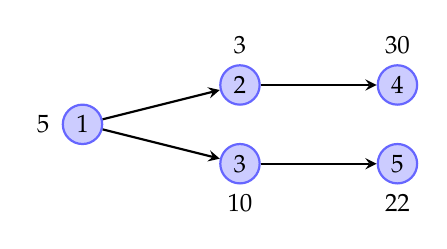
\begin{tikzpicture}
			[xscale=1.0,font=\small,
			node/.style={shape=circle,draw=blue!60,fill=blue!20,minimum
				width=.5cm,thick,inner sep=0pt}, arc/.style={->,>=stealth,thick}]       
			\node (1) [node] at (0,0) {$1$};
			\node (2) [node] at (2,.5) {$2$};
			\node (3) [node] at (2,-.5) {$3$};
			
			\node (4) [node] at (4,.5) {$4$};
			\node (5) [node] at (4,-.5) {$5$};
			
			\node at (-.5,0) {$5$};
			\node at (2,1) {$3$};
			\node at (2,-1) {$10$};
			\node at (4,1) {$30$};
			\node at (4,-1) {$22$};
			
			\draw [arc] (1) to (2);
			\draw [arc] (1) to (3);
			\draw [arc] (2) to (4);
			\draw [arc] (3) to (5);
			\end{tikzpicture}
		\end{center}
	\end{figure}
	The optimal multi-stage solution is $(6,(0,4),(24,12)$ with optimal cost of $36$;
	while two-stage optimal solution is $(10,0,20)$, with optimal cost of $40$.
	If we solve each path problem separately, we obtain optimal solutions for
	$P_1: (5,0,25)$ with cost 35, $P_2: (10,0,12)$ with cost $32$.
	{\color{blue}
	One thing to notice is that when enforcing non-anticipativity constraints,
	the model will somehow balance cost between paths. One consequence of such behavior
	is that the production at a certain node will cover more than what needed in this node
	but only fulfill partial demand of its children nodes.}
	
	If $d_4$ goes very large, $P_1$ will be the worst-case, thus multi-stage optimal
	solution will be $(5,(0,5),(d_4-5, 12)$; if $d_5$ becomes very large, the multi-stage
	optimal solution will be $(10,(0,0),(20,d-10)$. In either case, the two-stage optimal
	is always $(10,0,d-10)$.
\end{example}

Now let us take a look at an instance when costs are also uncertain.
The following example shows that the differences between the optimal costs of
two-stage and multi-stage formulations can be large due to the difference of
first-period decisions.
\begin{example}\label{ms-ts-diff2}
	Consider a three-period planning problem with one type of generator.
	Cost and demand data are as follows.
	\begin{figure}[htb]
		\begin{center}
			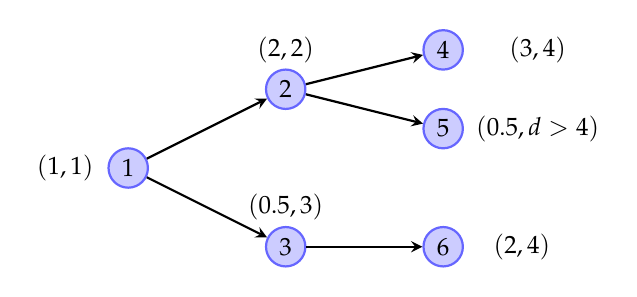
\begin{tikzpicture}
			[xscale=1.0,font=\small,
			node/.style={shape=circle,draw=blue!60,fill=blue!20,minimum
				width=.5cm,thick,inner sep=0pt}, arc/.style={->,>=stealth,thick}]       
			\node (1) [node] at (0,0) {$1$};
			\node (2) [node] at (2,1) {$2$};
			\node (3) [node] at (2,-1) {$3$};
			
			\node (4) [node] at (4,1.5) {$4$};
			\node (5) [node] at (4,0.5) {$5$};
			\node (6) [node] at (4,-1) {$6$};
			
			\node at (-.8,0) {$(1,1)$};
			\node at (2,1.5) {$(2,2)$};
			\node at (2,-.5) {$(0.5,3)$};
			\node at (5.2,1.5) {$(3,4)$};
			\node at (5.2,.5) {$(0.5,d>4)$};
			\node at (5,-1) {$(2,4)$};
			
			\draw [arc] (1) to (2);
			\draw [arc] (1) to (3);
			\draw [arc] (2) to (4);
			\draw [arc] (2) to (5);
			\draw [arc] (3) to (6);
			\end{tikzpicture}
		\end{center}
	\end{figure}
	The label beside each node represents the cost and demand realization pair.
	An optimal solution (the one optimal to DP formulation) to the multi-stage problem
	is $(2,(0,2),(2,d-2,0))$ with optimal worst-case cost $\frac{d+2}{2}$;
	while the optimal two-stage solution is $(d,0,0)$ with the optimal cost of $d$.
	
	{\color{blue} From this example, it looks like the difference in first-period decisions is affected by Node 5: those node with {\bf high demand but low cost}. In addition, the path that contains the node needs to be the worst-case path, otherwise,
	the decisions along that path may not affect the worst-case cost at all.}
\end{example}

\section*{March 12th, 2015}
Let us try to answer the second question \hyperref[qlist_1]{here}.
As we observed earlier, solving the multi-stage problem in one shot may produce a solution
that is not optimal at some part of the tree, so it does not make much sense to compare that solution with the stochastic optimal solution.
Therefore, we solve the multi-stage robust problem using PARU algorithm, then compare this solution with the optimal multi-stage stochastic solutions obtained by direct solving and PARU. Below are some computational results of small instances (here we use original scenario tree).

\noindent
\begin{minipage}[t]{8cm}
\tiny
\begin{verbatim}
Time horizon: 3
##################################################################
MS Robust MIP average: 2415.48
MS Robust MIP worstcase: 3587.98, Time used: 0.0937.
PARU - robust: first: 3587.98, last: 3587.98, Time used: 0.0937.
Put stochastic solution into robust model: 3587.98
Put PARU stochastic solution into robust model: 3587.98

MS Stochastic MIP: 2093.87, Time used: 0.0313.
PARU - stochastic: first: 2398.59, last: 2093.87, Time used: 0.078
Put robust solution into stochastic model: 2209.21
Put PARU robust solution into stochastic model: 2102.21

##################################################################
MS robust Integrality gap: 1.82%
TS-MS Gap (robust): 0.00%
TS-MS Gap (stochastic): 47.54%
MS-PARU Gap (robust): 0.00%
MS-PARU Gap (stochastic): 0.00%

##################################################################
MS robust solution - MS stochastic solution:
['                ', '                ', [0, 0, 0, 0, 0, 0]]
['                ', [0, 0, 0, 0, 0, 0], [0, -2, -1, 1, 0, 0]]
['                ', '                ', [0, -2, -1, 1, 0, 0]]
['                ', '                ', [0, 0, 0, 0, 0, 0]]
[[0, 0, 0, 0, 0, 0], [0, 1, -1, 0, 0, 0], [0, 1, -1, 0, 0, 0]]
['                ', '                ', [0, -1, 1, 0, 0, 0]]
['                ', '                ', [0, 0, 0, 0, 0, 0]]
['                ', [0, 0, 0, 0, 0, 0], [0, 0, 0, 0, 0, 0]]
['                ', '                ', [0, 0, 0, 0, 0, 0]]
MS robust solution - PARU robust solution:
['                ', '                ', [0, 0, 0, 0, 0, 0]]
['                ', [0, 0, 0, 0, 0, 0], [0, -2, -1, 1, 0, 0]]
['                ', '                ', [0, -2, -1, 1, 0, 0]]
['                ', '                ', [0, 0, 0, 0, 0, 0]]
[[0, 0, 0, 0, 0, 0], [0, 1, -1, 0, 0, 0], [0, 0, 0, 0, 0, 0]]
['                ', '                ', [0, -1, 1, 0, 0, 0]]
['                ', '                ', [0, 0, 0, 0, 0, 0]]
['                ', [0, 0, 0, 0, 0, 0], [0, -1, 1, 0, 0, 0]]
['                ', '                ', [0, 0, 0, 0, 0, 0]]
MS robust solution - PARU stochastic solution:
['                ', '                ', [0, 0, 0, 0, 0, 0]]
['                ', [0, 0, 0, 0, 0, 0], [0, -2, -1, 1, 0, 0]]
['                ', '                ', [0, -2, -1, 1, 0, 0]]
['                ', '                ', [0, 0, 0, 0, 0, 0]]
[[0, 0, 0, 0, 0, 0], [0, 1, -1, 0, 0, 0], [0, 1, -1, 0, 0, 0]]
['                ', '                ', [0, -1, 1, 0, 0, 0]]
['                ', '                ', [0, 0, 0, 0, 0, 0]]
['                ', [0, 0, 0, 0, 0, 0], [0, 0, 0, 0, 0, 0]]
['                ', '                ', [0, 0, 0, 0, 0, 0]]
MS stochastic solution - PARU stochastic solution:
['                ', '                ', [0, 0, 0, 0, 0, 0]]
['                ', [0, 0, 0, 0, 0, 0], [0, 0, 0, 0, 0, 0]]
['                ', '                ', [0, 0, 0, 0, 0, 0]]
['                ', '                ', [0, 0, 0, 0, 0, 0]]
[[0, 0, 0, 0, 0, 0], [0, 0, 0, 0, 0, 0], [0, 0, 0, 0, 0, 0]]
['                ', '                ', [0, 0, 0, 0, 0, 0]]
['                ', '                ', [0, 0, 0, 0, 0, 0]]
['                ', [0, 0, 0, 0, 0, 0], [0, 0, 0, 0, 0, 0]]
['                ', '                ', [0, 0, 0, 0, 0, 0]]
MS stochastic solution - PARU robust solution:
['                ', '                ', [0, 0, 0, 0, 0, 0]]
['                ', [0, 0, 0, 0, 0, 0], [0, 0, 0, 0, 0, 0]]
['                ', '                ', [0, 0, 0, 0, 0, 0]]
['                ', '                ', [0, 0, 0, 0, 0, 0]]
[[0, 0, 0, 0, 0, 0], [0, 0, 0, 0, 0, 0], [0, -1, 1, 0, 0, 0]]
['                ', '                ', [0, 0, 0, 0, 0, 0]]
['                ', '                ', [0, 0, 0, 0, 0, 0]]
['                ', [0, 0, 0, 0, 0, 0], [0, -1, 1, 0, 0, 0]]
['                ', '                ', [0, 0, 0, 0, 0, 0]]
\end{verbatim}
\end{minipage}
\begin{minipage}[t]{8cm}
\tiny
\begin{verbatim}
##################################################################
MS robust solution:
['                ', '                ', [0, 0, 0, 0, 0, 0]]
['                ', [0, 0, 0, 0, 0, 0], [0, 0, 0, 1, 0, 0]]
['                ', '                ', [0, 0, 0, 1, 0, 0]]
['                ', '                ', [0, 0, 0, 0, 0, 0]]
[[0, 0, 0, 0, 0, 0], [0, 1, 0, 1, 0, 0], [0, 3, 0, 0, 0, 0]]
['                ', '                ', [0, 1, 2, 0, 0, 0]]
['                ', '                ', [0, 0, 0, 0, 0, 0]]
['                ', [0, 0, 1, 1, 0, 0], [0, 2, 1, 0, 0, 0]]
['                ', '                ', [0, 3, 0, 0, 0, 0]]
PARU robust solution:
['                ', '                ', [0, 0, 0, 0, 0, 0]]
['                ', [0, 0, 0, 0, 0, 0], [0, 2, 1, 0, 0, 0]]
['                ', '                ', [0, 2, 1, 0, 0, 0]]
['                ', '                ', [0, 0, 0, 0, 0, 0]]
[[0, 0, 0, 0, 0, 0], [0, 0, 1, 1, 0, 0], [0, 3, 0, 0, 0, 0]]
['                ', '                ', [0, 2, 1, 0, 0, 0]]
['                ', '                ', [0, 0, 0, 0, 0, 0]]
['                ', [0, 0, 1, 1, 0, 0], [0, 3, 0, 0, 0, 0]]
['                ', '                ', [0, 3, 0, 0, 0, 0]]
MS stochastic solution:
['                ', '                ', [0, 0, 0, 0, 0, 0]]
['                ', [0, 0, 0, 0, 0, 0], [0, 2, 1, 0, 0, 0]]
['                ', '                ', [0, 2, 1, 0, 0, 0]]
['                ', '                ', [0, 0, 0, 0, 0, 0]]
[[0, 0, 0, 0, 0, 0], [0, 0, 1, 1, 0, 0], [0, 2, 1, 0, 0, 0]]
['                ', '                ', [0, 2, 1, 0, 0, 0]]
['                ', '                ', [0, 0, 0, 0, 0, 0]]
['                ', [0, 0, 1, 1, 0, 0], [0, 2, 1, 0, 0, 0]]
['                ', '                ', [0, 3, 0, 0, 0, 0]]
PARU stochastic solution:
['                ', '                ', [0, 0, 0, 0, 0, 0]]
['                ', [0, 0, 0, 0, 0, 0], [0, 2, 1, 0, 0, 0]]
['                ', '                ', [0, 2, 1, 0, 0, 0]]
['                ', '                ', [0, 0, 0, 0, 0, 0]]
[[0, 0, 0, 0, 0, 0], [0, 0, 1, 1, 0, 0], [0, 2, 1, 0, 0, 0]]
['                ', '                ', [0, 2, 1, 0, 0, 0]]
['                ', '                ', [0, 0, 0, 0, 0, 0]]
['                ', [0, 0, 1, 1, 0, 0], [0, 2, 1, 0, 0, 0]]
['                ', '                ', [0, 3, 0, 0, 0, 0]]
\end{verbatim}
\end{minipage}

\begin{minipage}[t]{9cm}
\tiny
\begin{verbatim}
Time horizon: 4
##################################################################
MS Robust MIP average: 4782.81
MS Robust MIP worstcase: 6063.53, Time used: 1.8136.
PARU - robust: first: 6063.53, last: 6063.53, Time used: 0.7188.
Put stochastic solution into robust model: 6069.42
Put PARU stochastic solution into robust model: 6069.42

MS Stochastic MIP: 3107.09, Time used: 1.1021.
PARU - stochastic: first: 3920.42, last: 3107.09, Time used: 6.8609.
Put robust solution into stochastic model: 4461.35
Put PARU robust solution into stochastic model: 3303.54

##################################################################
MS robust Integrality gap: 1.68%
TS-MS Gap (robust): 0.00%
TS-MS Gap (stochastic): 42.81%
MS-PARU Gap (robust): -0.00%
MS-PARU Gap (stochastic): 0.00%

##################################################################
MS robust solution - MS stochastic solution:
['                ', '                ', '                ', [0, 0, 0, 0, 0, 0]]
['                ', '                ', [0, 0, 0, 1, 0, 0], [0, -1, 0, 0, 0, 0]]
['                ', '                ', '                ', [0, -1, -1, 0, 0, 0]]
['                ', '                ', '                ', [0, 0, 0, 0, 0, 0]]
['                ', [0, 0, 0, 0, 0, 0], [2, 0, 0, 0, 0, 0], [0, -1, -1, 0, 0, 0]]
['                ', '                ', '                ', [0, -1, -2, 0, 0, 0]]
['                ', '                ', '                ', [0, 0, 0, 0, 0, 0]]
['                ', '                ', [0, 0, 0, 0, 0, 0], [0, -2, -1, 0, 6, 0]]
['                ', '                ', '                ', [0, -2, 5, 0, 0, 0]]
['                ', '                ', '                ', [0, 0, 2, 0, 0, 0]]
['                ', '                ', [0, 0, 0, 0, 0, 1], [0, 5, -1, 0, 0, 0]]
['                ', '                ', '                ', [0, 5, -1, 0, 0, 0]]
['                ', '                ', '                ', [0, 0, 0, 0, 1, 1]]
[[0, 0, 0, 0, 0, 0], [0, 0, 0, 0, 0, 0], [0, -1, 2, 0, 0, 1], [0, -1, 0, 0, 0, 0]]
['                ', '                ', '                ', [0, -1, -1, 0, 0, 0]]
['                ', '                ', '                ', [0, 0, 6, 0, 0, 0]]
['                ', '                ', [0, -1, 1, 0, 0, 0], [0, -1, -1, 0, 0, 1]]
['                ', '                ', '                ', [0, 2, -2, 0, 0, 0]]
['                ', '                ', '                ', [0, 0, 0, 0, 0, 0]]
['                ', '                ', [0, 0, 0, 0, 0, 0], [0, -2, 0, 0, 6, 0]]
['                ', '                ', '                ', [0, -2, 0, 0, 6, 0]]
['                ', '                ', '                ', [0, 6, 0, 0, 0, 0]]
['                ', [0, 1, -1, 0, 0, 0], [0, -2, 1, 0, 0, 1], [0, 0, -1, 0, 0, 0]]
['                ', '                ', '                ', [0, 0, -1, 0, 0, 0]]
['                ', '                ', '                ', [0, 0, 0, 0, 0, 0]]
['                ', '                ', [0, 0, 0, 0, 0, 0], [0, -1, 1, 0, 0, 0]]
['                ', '                ', '                ', [0, -1, 1, 0, 0, 0]]
MS robust solution - PARU robust solution:
['                ', '                ', '                ', [0, 0, 0, 0, 0, 0]]
['                ', '                ', [0, 0, 0, 1, 0, 0], [0, -1, 0, 0, 0, 0]]
['                ', '                ', '                ', [0, -1, -1, 0, 0, 0]]
['                ', '                ', '                ', [0, 0, 0, 0, 0, 0]]
['                ', [0, 0, 0, 0, 0, 0], [2, 0, 0, 0, 0, 0], [0, -2, 0, 0, 0, 0]]
['                ', '                ', '                ', [0, -1, -2, 0, 0, 0]]
['                ', '                ', '                ', [0, -2, 0, 0, 0, 0]]
['                ', '                ', [0, 0, 0, 0, 0, 0], [0, -2, -1, 0, 6, 0]]
['                ', '                ', '                ', [0, -2, 5, 0, 0, 0]]
['                ', '                ', '                ', [0, 0, 2, 0, 0, 0]]
['                ', '                ', [0, 0, 0, 0, 0, 1], [0, 5, -1, 0, 0, 0]]
['                ', '                ', '                ', [0, 5, -1, 0, 0, 0]]
['                ', '                ', '                ', [0, -1, 0, 0, 1, 1]]
[[0, 0, 0, 0, 0, 0], [0, 0, 0, 0, 0, 0], [0, -1, 3, 0, 0, 0], [0, 1, -2, 0, 0, 0]]
['                ', '                ', '                ', [0, 1, -2, 0, 0, 0]]
['                ', '                ', '                ', [0, -5, 6, 0, 0, 0]]
['                ', '                ', [0, 0, 1, 0, 0, -1], [0, -1, 0, 0, 0, 1]]
['                ', '                ', '                ', [0, 2, -1, 0, 0, 0]]
['                ', '                ', '                ', [0, 0, 0, 0, 0, 0]]
['                ', '                ', [0, 0, 0, 0, 0, 0], [0, 0, -2, 0, 6, 0]]
['                ', '                ', '                ', [0, -1, -1, 0, 6, 0]]
['                ', '                ', '                ', [0, 6, 0, 0, 0, 0]]
['                ', [0, 0, 0, 0, 0, 0], [0, 0, 0, 0, 0, 0], [0, 0, 0, 0, 0, 0]]
['                ', '                ', '                ', [0, 0, 0, 0, 0, 0]]
['                ', '                ', '                ', [0, 0, 0, 0, -1, 0]]
['                ', '                ', [0, 0, 0, 0, 0, 0], [0, 0, 0, 0, 0, 0]]
['                ', '                ', '                ', [0, 0, 0, 0, 0, 0]]
MS robust solution - PARU stochastic solution:
['                ', '                ', '                ', [0, 0, 0, 0, 0, 0]]
['                ', '                ', [0, 0, 0, 1, 0, 0], [0, -1, 0, 0, 0, 0]]
['                ', '                ', '                ', [0, -1, -1, 0, 0, 0]]
['                ', '                ', '                ', [0, 0, 0, 0, 0, 0]]
['                ', [0, 0, 0, 0, 0, 0], [2, 0, 0, 0, 0, 0], [0, -1, -1, 0, 0, 0]]
['                ', '                ', '                ', [0, -1, -2, 0, 0, 0]]
['                ', '                ', '                ', [0, 0, 0, 0, 0, 0]]
['                ', '                ', [0, 0, 0, 0, 0, 0], [0, -2, -1, 0, 6, 0]]
['                ', '                ', '                ', [0, -2, 5, 0, 0, 0]]
['                ', '                ', '                ', [0, 0, 2, 0, 0, 0]]
['                ', '                ', [0, 0, 0, 0, 0, 1], [0, 5, -1, 0, 0, 0]]
['                ', '                ', '                ', [0, 5, -1, 0, 0, 0]]
['                ', '                ', '                ', [0, 0, 0, 0, 1, 1]]
[[0, 0, 0, 0, 0, 0], [0, 0, 0, 0, 0, 0], [0, -1, 2, 0, 0, 1], [0, -1, 0, 0, 0, 0]]
['                ', '                ', '                ', [0, -1, -1, 0, 0, 0]]
['                ', '                ', '                ', [0, 0, 6, 0, 0, 0]]
['                ', '                ', [0, -1, 1, 0, 0, 0], [0, -1, -1, 0, 0, 1]]
['                ', '                ', '                ', [0, 2, -2, 0, 0, 0]]
['                ', '                ', '                ', [0, 0, 0, 0, 0, 0]]
['                ', '                ', [0, 0, 0, 0, 0, 0], [0, -2, 0, 0, 6, 0]]
['                ', '                ', '                ', [0, -2, 0, 0, 6, 0]]
['                ', '                ', '                ', [0, 6, 0, 0, 0, 0]]
['                ', [0, 1, -1, 0, 0, 0], [0, -2, 1, 0, 0, 1], [0, 0, -1, 0, 0, 0]]
['                ', '                ', '                ', [0, 0, -1, 0, 0, 0]]
['                ', '                ', '                ', [0, 0, 0, 0, 0, 0]]
['                ', '                ', [0, 0, 0, 0, 0, 0], [0, -1, 1, 0, 0, 0]]
['                ', '                ', '                ', [0, -1, 1, 0, 0, 0]]
\end{verbatim}
\end{minipage}
\begin{minipage}[t]{8cm}
\tiny
\begin{verbatim}
MS stochastic solution - PARU stochastic solution:
['                ', '                ', '                ', [0, 0, 0, 0, 0, 0]]
['                ', '                ', [0, 0, 0, 0, 0, 0], [0, 0, 0, 0, 0, 0]]
['                ', '                ', '                ', [0, 0, 0, 0, 0, 0]]
['                ', '                ', '                ', [0, 0, 0, 0, 0, 0]]
['                ', [0, 0, 0, 0, 0, 0], [0, 0, 0, 0, 0, 0], [0, 0, 0, 0, 0, 0]]
['                ', '                ', '                ', [0, 0, 0, 0, 0, 0]]
['                ', '                ', '                ', [0, 0, 0, 0, 0, 0]]
['                ', '                ', [0, 0, 0, 0, 0, 0], [0, 0, 0, 0, 0, 0]]
['                ', '                ', '                ', [0, 0, 0, 0, 0, 0]]
['                ', '                ', '                ', [0, 0, 0, 0, 0, 0]]
['                ', '                ', [0, 0, 0, 0, 0, 0], [0, 0, 0, 0, 0, 0]]
['                ', '                ', '                ', [0, 0, 0, 0, 0, 0]]
['                ', '                ', '                ', [0, 0, 0, 0, 0, 0]]
[[0, 0, 0, 0, 0, 0], [0, 0, 0, 0, 0, 0], [0, 0, 0, 0, 0, 0], [0, 0, 0, 0, 0, 0]]
['                ', '                ', '                ', [0, 0, 0, 0, 0, 0]]
['                ', '                ', '                ', [0, 0, 0, 0, 0, 0]]
['                ', '                ', [0, 0, 0, 0, 0, 0], [0, 0, 0, 0, 0, 0]]
['                ', '                ', '                ', [0, 0, 0, 0, 0, 0]]
['                ', '                ', '                ', [0, 0, 0, 0, 0, 0]]
['                ', '                ', [0, 0, 0, 0, 0, 0], [0, 0, 0, 0, 0, 0]]
['                ', '                ', '                ', [0, 0, 0, 0, 0, 0]]
['                ', '                ', '                ', [0, 0, 0, 0, 0, 0]]
['                ', [0, 0, 0, 0, 0, 0], [0, 0, 0, 0, 0, 0], [0, 0, 0, 0, 0, 0]]
['                ', '                ', '                ', [0, 0, 0, 0, 0, 0]]
['                ', '                ', '                ', [0, 0, 0, 0, 0, 0]]
['                ', '                ', [0, 0, 0, 0, 0, 0], [0, 0, 0, 0, 0, 0]]
['                ', '                ', '                ', [0, 0, 0, 0, 0, 0]]
MS stochastic solution - PARU robust solution:
['                ', '                ', '                ', [0, 0, 0, 0, 0, 0]]
['                ', '                ', [0, 0, 0, 0, 0, 0], [0, 0, 0, 0, 0, 0]]
['                ', '                ', '                ', [0, 0, 0, 0, 0, 0]]
['                ', '                ', '                ', [0, 0, 0, 0, 0, 0]]
['                ', [0, 0, 0, 0, 0, 0], [0, 0, 0, 0, 0, 0], [0, -1, 1, 0, 0, 0]]
['                ', '                ', '                ', [0, 0, 0, 0, 0, 0]]
['                ', '                ', '                ', [0, -2, 0, 0, 0, 0]]
['                ', '                ', [0, 0, 0, 0, 0, 0], [0, 0, 0, 0, 0, 0]]
['                ', '                ', '                ', [0, 0, 0, 0, 0, 0]]
['                ', '                ', '                ', [0, 0, 0, 0, 0, 0]]
['                ', '                ', [0, 0, 0, 0, 0, 0], [0, 0, 0, 0, 0, 0]]
['                ', '                ', '                ', [0, 0, 0, 0, 0, 0]]
['                ', '                ', '                ', [0, -1, 0, 0, 0, 0]]
[[0, 0, 0, 0, 0, 0], [0, 0, 0, 0, 0, 0], [0, 0, 1, 0, 0, -1], [0, 2, -2, 0, 0, 0]]
['                ', '                ', '                ', [0, 2, -1, 0, 0, 0]]
['                ', '                ', '                ', [0, -5, 0, 0, 0, 0]]
['                ', '                ', [0, 1, 0, 0, 0, -1], [0, 0, 1, 0, 0, 0]]
['                ', '                ', '                ', [0, 0, 1, 0, 0, 0]]
['                ', '                ', '                ', [0, 0, 0, 0, 0, 0]]
['                ', '                ', [0, 0, 0, 0, 0, 0], [0, 2, -2, 0, 0, 0]]
['                ', '                ', '                ', [0, 1, -1, 0, 0, 0]]
['                ', '                ', '                ', [0, 0, 0, 0, 0, 0]]
['                ', [0, -1, 1, 0, 0, 0], [0, 2, -1, 0, 0, -1], [0, 0, 1, 0, 0, 0]]
['                ', '                ', '                ', [0, 0, 1, 0, 0, 0]]
['                ', '                ', '                ', [0, 0, 0, 0, -1, 0]]
['                ', '                ', [0, 0, 0, 0, 0, 0], [0, 1, -1, 0, 0, 0]]
['                ', '                ', '                ', [0, 1, -1, 0, 0, 0]]
##################################################################
MS robust solution:
['                ', '                ', '                ', [0, 0, 0, 0, 0, 0]]
['                ', '                ', [0, 0, 0, 1, 0, 0], [0, 0, 0, 0, 0, 0]]
['                ', '                ', '                ', [0, 0, 0, 0, 0, 0]]
['                ', '                ', '                ', [0, 0, 0, 0, 0, 0]]
['                ', [0, 0, 0, 0, 0, 0], [2, 0, 0, 1, 0, 0], [0, 0, 1, 0, 0, 0]]
['                ', '                ', '                ', [0, 0, 0, 0, 0, 0]]
['                ', '                ', '                ', [0, 0, 0, 0, 0, 0]]
['                ', '                ', [0, 0, 0, 1, 0, 0], [0, 0, 0, 0, 6, 0]]
['                ', '                ', '                ', [0, 0, 6, 0, 0, 0]]
['                ', '                ', '                ', [0, 0, 2, 0, 0, 0]]
['                ', '                ', [0, 0, 0, 0, 0, 1], [0, 6, 0, 0, 0, 0]]
['                ', '                ', '                ', [0, 6, 0, 0, 0, 0]]
['                ', '                ', '                ', [0, 0, 0, 0, 1, 1]]
[[0, 0, 0, 0, 0, 0], [0, 0, 1, 1, 0, 0], [0, 1, 3, 0, 0, 1], [0, 2, 0, 0, 0, 0]]
['                ', '                ', '                ', [0, 2, 0, 0, 0, 0]]
['                ', '                ', '                ', [0, 0, 6, 0, 0, 0]]
['                ', '                ', [0, 2, 1, 0, 0, 0], [0, 1, 1, 0, 0, 1]]
['                ', '                ', '                ', [0, 4, 0, 0, 0, 0]]
['                ', '                ', '                ', [0, 0, 0, 0, 0, 0]]
['                ', '                ', [0, 0, 0, 0, 0, 0], [0, 0, 0, 0, 6, 0]]
['                ', '                ', '                ', [0, 0, 0, 0, 6, 0]]
['                ', '                ', '                ', [0, 6, 0, 0, 0, 0]]
['                ', [0, 1, 0, 1, 0, 0], [0, 1, 1, 0, 0, 1], [0, 2, 1, 0, 0, 0]]
['                ', '                ', '                ', [0, 2, 1, 0, 0, 0]]
['                ', '                ', '                ', [0, 0, 0, 0, 0, 0]]
['                ', '                ', [0, 3, 0, 0, 0, 0], [0, 1, 3, 0, 0, 0]]
['                ', '                ', '                ', [0, 1, 3, 0, 0, 0]]
PARU robust solution:
['                ', '                ', '                ', [0, 0, 0, 0, 0, 0]]
['                ', '                ', [0, 0, 0, 0, 0, 0], [0, 1, 0, 0, 0, 0]]
['                ', '                ', '                ', [0, 1, 1, 0, 0, 0]]
['                ', '                ', '                ', [0, 0, 0, 0, 0, 0]]
['                ', [0, 0, 0, 0, 0, 0], [0, 0, 0, 1, 0, 0], [0, 2, 1, 0, 0, 0]]
['                ', '                ', '                ', [0, 1, 2, 0, 0, 0]]
['                ', '                ', '                ', [0, 2, 0, 0, 0, 0]]
['                ', '                ', [0, 0, 0, 1, 0, 0], [0, 2, 1, 0, 0, 0]]
['                ', '                ', '                ', [0, 2, 1, 0, 0, 0]]
['                ', '                ', '                ', [0, 0, 0, 0, 0, 0]]
['                ', '                ', [0, 0, 0, 0, 0, 0], [0, 1, 1, 0, 0, 0]]
['                ', '                ', '                ', [0, 1, 1, 0, 0, 0]]
['                ', '                ', '                ', [0, 1, 0, 0, 0, 0]]
[[0, 0, 0, 0, 0, 0], [0, 0, 1, 1, 0, 0], [0, 2, 0, 0, 0, 1], [0, 1, 2, 0, 0, 0]]
['                ', '                ', '                ', [0, 1, 2, 0, 0, 0]]
['                ', '                ', '                ', [0, 5, 0, 0, 0, 0]]
['                ', '                ', [0, 2, 0, 0, 0, 1], [0, 2, 1, 0, 0, 0]]
['                ', '                ', '                ', [0, 2, 1, 0, 0, 0]]
['                ', '                ', '                ', [0, 0, 0, 0, 0, 0]]
['                ', '                ', [0, 0, 0, 0, 0, 0], [0, 0, 2, 0, 0, 0]]
['                ', '                ', '                ', [0, 1, 1, 0, 0, 0]]
['                ', '                ', '                ', [0, 0, 0, 0, 0, 0]]
['                ', [0, 1, 0, 1, 0, 0], [0, 1, 1, 0, 0, 1], [0, 2, 1, 0, 0, 0]]
['                ', '                ', '                ', [0, 2, 1, 0, 0, 0]]
['                ', '                ', '                ', [0, 0, 0, 0, 1, 0]]
['                ', '                ', [0, 3, 0, 0, 0, 0], [0, 1, 3, 0, 0, 0]]
['                ', '                ', '                ', [0, 1, 3, 0, 0, 0]]
\end{verbatim}
\end{minipage}
\begin{minipage}[t]{9cm}\tiny
	\begin{verbatim}
	MS stochastic solution:
	['                ', '                ', '                ', [0, 0, 0, 0, 0, 0]]
	['                ', '                ', [0, 0, 0, 0, 0, 0], [0, 1, 0, 0, 0, 0]]
	['                ', '                ', '                ', [0, 1, 1, 0, 0, 0]]
	['                ', '                ', '                ', [0, 0, 0, 0, 0, 0]]
	['                ', [0, 0, 0, 0, 0, 0], [0, 0, 0, 1, 0, 0], [0, 1, 2, 0, 0, 0]]
	['                ', '                ', '                ', [0, 1, 2, 0, 0, 0]]
	['                ', '                ', '                ', [0, 0, 0, 0, 0, 0]]
	['                ', '                ', [0, 0, 0, 1, 0, 0], [0, 2, 1, 0, 0, 0]]
	['                ', '                ', '                ', [0, 2, 1, 0, 0, 0]]
	['                ', '                ', '                ', [0, 0, 0, 0, 0, 0]]
	['                ', '                ', [0, 0, 0, 0, 0, 0], [0, 1, 1, 0, 0, 0]]
	['                ', '                ', '                ', [0, 1, 1, 0, 0, 0]]
	['                ', '                ', '                ', [0, 0, 0, 0, 0, 0]]
	[[0, 0, 0, 0, 0, 0], [0, 0, 1, 1, 0, 0], [0, 2, 1, 0, 0, 0], [0, 3, 0, 0, 0, 0]]
	['                ', '                ', '                ', [0, 3, 1, 0, 0, 0]]
	['                ', '                ', '                ', [0, 0, 0, 0, 0, 0]]
	['                ', '                ', [0, 3, 0, 0, 0, 0], [0, 2, 2, 0, 0, 0]]
	['                ', '                ', '                ', [0, 2, 2, 0, 0, 0]]
	['                ', '                ', '                ', [0, 0, 0, 0, 0, 0]]
	['                ', '                ', [0, 0, 0, 0, 0, 0], [0, 2, 0, 0, 0, 0]]
	['                ', '                ', '                ', [0, 2, 0, 0, 0, 0]]
	['                ', '                ', '                ', [0, 0, 0, 0, 0, 0]]
	['                ', [0, 0, 1, 1, 0, 0], [0, 3, 0, 0, 0, 0], [0, 2, 2, 0, 0, 0]]
	['                ', '                ', '                ', [0, 2, 2, 0, 0, 0]]
	['                ', '                ', '                ', [0, 0, 0, 0, 0, 0]]
	['                ', '                ', [0, 3, 0, 0, 0, 0], [0, 2, 2, 0, 0, 0]]
	['                ', '                ', '                ', [0, 2, 2, 0, 0, 0]]
	\end{verbatim}
\end{minipage}
\begin{minipage}[t]{9cm}\tiny
	\begin{verbatim}
PARU stochastic solution:
['                ', '                ', '                ', [0, 0, 0, 0, 0, 0]]
['                ', '                ', [0, 0, 0, 0, 0, 0], [0, 1, 0, 0, 0, 0]]
['                ', '                ', '                ', [0, 1, 1, 0, 0, 0]]
['                ', '                ', '                ', [0, 0, 0, 0, 0, 0]]
['                ', [0, 0, 0, 0, 0, 0], [0, 0, 0, 1, 0, 0], [0, 1, 2, 0, 0, 0]]
['                ', '                ', '                ', [0, 1, 2, 0, 0, 0]]
['                ', '                ', '                ', [0, 0, 0, 0, 0, 0]]
['                ', '                ', [0, 0, 0, 1, 0, 0], [0, 2, 1, 0, 0, 0]]
['                ', '                ', '                ', [0, 2, 1, 0, 0, 0]]
['                ', '                ', '                ', [0, 0, 0, 0, 0, 0]]
['                ', '                ', [0, 0, 0, 0, 0, 0], [0, 1, 1, 0, 0, 0]]
['                ', '                ', '                ', [0, 1, 1, 0, 0, 0]]
['                ', '                ', '                ', [0, 0, 0, 0, 0, 0]]
[[0, 0, 0, 0, 0, 0], [0, 0, 1, 1, 0, 0], [0, 2, 1, 0, 0, 0], [0, 3, 0, 0, 0, 0]]
['                ', '                ', '                ', [0, 3, 1, 0, 0, 0]]
['                ', '                ', '                ', [0, 0, 0, 0, 0, 0]]
['                ', '                ', [0, 3, 0, 0, 0, 0], [0, 2, 2, 0, 0, 0]]
['                ', '                ', '                ', [0, 2, 2, 0, 0, 0]]
['                ', '                ', '                ', [0, 0, 0, 0, 0, 0]]
['                ', '                ', [0, 0, 0, 0, 0, 0], [0, 2, 0, 0, 0, 0]]
['                ', '                ', '                ', [0, 2, 0, 0, 0, 0]]
['                ', '                ', '                ', [0, 0, 0, 0, 0, 0]]
['                ', [0, 0, 1, 1, 0, 0], [0, 3, 0, 0, 0, 0], [0, 2, 2, 0, 0, 0]]
['                ', '                ', '                ', [0, 2, 2, 0, 0, 0]]
['                ', '                ', '                ', [0, 0, 0, 0, 0, 0]]
['                ', '                ', [0, 3, 0, 0, 0, 0], [0, 2, 2, 0, 0, 0]]
['                ', '                ', '                ', [0, 2, 2, 0, 0, 0]]
\end{verbatim}
\end{minipage}

\subsection*{Summary from computational results}
\begin{enumerate}
	\item The worst case is always the last path in these instances. This is due to the dataset used in the test.
	\item The optimal multi-stage stochastic solution and the multi-stage robust solution
	obtained by PARU are similar.
\end{enumerate}

\section*{March 17th, 2015}
For the simplified problem, i.e., the problem with only $x$-variables in 1-dimension,
we have known that the solution obtained by MIP solver is not necessarily DP-optimal,
as mentioned in \citet{bertsimas2010optimality}. However, we can show that even though
the entire solution is not DP-optimal, the first-period solution is DP-optimal.
\begin{proposition}
	{\color{blue}There exists one optimal solution to the DP formulation such that the first-period decision coincides with that in each optimal solution which is not DP-optimal.}
\end{proposition}
\begin{proof}~
	Suppose there exists an optimal solution $\hat{\bx}$ to the finite adaptive formulation
	such that no DP-optimal solution shares the same first-period decision.
	Let $v^*$ be the DP optimal value and $v(\bx)$ be the worst-case cost given by the
	solution $\bx$. In addition, let $v^{DP}(x_1)$ be the worst-case cost given by solving
	a DP formulation with first-period decision fixed at $x_1$. Therefore,
	we have the following inequality series:
	\[v(\hat{x}) = v^* > v^{DP}(\hat{x}_1) \ge v(\hat{x}).\]
	The first strict inequality is due to the assumption that no DP-optimal solution
	shares the same first-period decision as $\hat{x}_1$. The second inequality is due
	to the fact that the obtained DP solution is feasible to the original multi-stage formulation.
\end{proof}

{\color{red}
	The optimal solution to the DP formulation is time consistent since the risk measure is the worst-case risk measure \citep{shapiro2012time}.
	But the inconsistency we have seen is not brought by the risk measure but the formulation itself. It could be interesting if one can come up with a formulation
	that enforce the consistency.
}

\citet{iancu2013pareto} discussed a notion called \emph{Pareto efficiency} 
in robust optimization. Due to the fact that there may be multiple robust optimal solutions, is there an robust optimal solution that Pareto dominates any other optimal solutions? That is, for any uncertainty realization other than the worst case scenario, such solution also yields
the best possible objective function value among all robust optimal solutions.
They show that for robust linear problems, such solution always exists, but
may form a nonconvex set. It is also possible to compute such a solution
without increasing the computational complexity of the computing robust optimal solutions.
{\color{red}What does Pareto efficiency mean in our problem?}
\section*{March 19th, 2015}
Consider the following primal and dual pair.

\begin{minipage}{0.5\textwidth}
	\begin{align*}
	[P]\quad \min \quad & \theta\\
	\subjectto\quad & \theta \ge \sum_{n\in P}c_nx_n, \quad \forall P\in \cP\\
	& \sum_{m\in P(n)}x_m \ge d_n,\quad \forall n\in \T\\
	& x_n\ge 0, \quad \forall n\in \T.
	\end{align*}
\end{minipage}
\begin{minipage}{0.5\textwidth}
	\begin{align*}
	[D]\quad \max \quad & \sum_{n\in \T}d_n\beta_n\\
	\subjectto\quad & \sum_{m\in T(n)}\beta_m - c_n\sum_{P:n\in P}\alpha_P \le 0, \quad \forall n\in \T\\
	& \sum_{P\in \cP}\alpha_P = 1\\
	& \beta_n\ge 0, \alpha_P\ge 0, \quad \forall n\in \T, P\in \cP.
	\end{align*}
\end{minipage}

From the dual, we notice that for $n\in \T$, we have,
\[0\le \beta_n \le \min_{m\in P(n)}\left\{ c_m\sum_{P:m\in P}\alpha_P - \sum_{k\in T(m)\setminus \{n\}}\beta_k\right\}.\]
With a DP optimal solution, it could be possible that there are more
than one tight path. Thus the dual optimal solution may have more than
$\alpha_P$ being positive. This brings difficulty in constructing optimal 
solutions from the dual problem.

Let's focus on the primal problem. Consider the following example.
First part of the tableau shows the (cost,demand) pair.
The second and the third part contains the DP optimal solution to the LP
relaxation and original problem, respectively.

\begin{tabular}{ccc||}
        &		   & (1,\;11)\\
	    & (6,\;2)  & (7,\;10)\\
	    &		   & (2,\;12)\\
	    &		   & (9,\;14)\\
(5,\;1) & (10,\;3) & (8,\;16)\\
	    &		   & (2,\;16)\\
	    &		   & (6,\;18)\\
	    & (3,\;4)  & (2,\;19)\\
	    &		   & (5,\;20)
\end{tabular}
\begin{tabular}{ccc c||}
	 &	   & 0 & (68)\\
	 & 0   & 0 & (68)\\
	 &	   & 0 & (68)\\
	 &	   & 0.4 & (71.6)\\
13.6 & 0   & 2.4 & ({\color{red}87.2})\\
	 &	   & 2.4 & (72.8) \\
	 &	   & 0 & ({\color{red}87.2})\\
	 & 6.4 & 0 & ({\color{red}87.2})\\
	 & 	   & 0 & ({\color{red}87.2})
\end{tabular}
\begin{tabular}{ccc c||}
	&	 & 0 & (70)\\
	& 0  & 0 & (70)\\
	&	 & 0 & (70)\\
	&	 & 0 & (70)\\
14	& 0  & 2 & (86)\\
	&	 & 2 & (74) \\
	&	 & 0 & ({\color{red}88})\\
	& 6  & 0 & ({\color{red}88})\\
	& 	 & 0 & ({\color{red}88})
\end{tabular}

\begin{algorithm}
\caption{A primal algorithm}
\label{alg:primal}
\begin{algorithmic}[1]
\STATE Set $\hat{x}_n = (d_n-\sum_{m\in P(a(n))}x_m)_+$ for $n=1\dots, N$ sequentially
\STATE $k\gets \max\{n\in \T: T(n)\setminus \{n\} \neq \emptyset\}$
\WHILE{$k \ge 0$}
\STATE Calculate the cost of each path in $T(k)$
\STATE $k\gets k-1$
\ENDWHILE
\end{algorithmic}
\end{algorithm}
In the above example, Step 1 produces (parenthesis contains unitcost-production pair)

\noindent\begin{tabular}{ccc c||}
$T=1$ & $T=2$ & $T=3$ & path cost from t2\\
        &		   & (1,\;9) & (15)\\
        & (6,\;1)  & (7,\;8) & (62)\\
        &		   & (2,\;10)& (26)\\
        &		   & (9,\;11)& ({\color{blue}119})\\
(5,\;1) & (10,\;2) & (8,\;13)& ({\color{blue}124})\\
        &		   & (2,\;13)& ({\color{blue}46})\\
        &		   & (6,\;14)& ({\color{red}93})\\
        & (3,\;3)  & (2,\;15)& ({\color{red}39})\\
        &		   & (5,\;16)& ({\color{red}89})
\end{tabular}
\begin{minipage}{0.5\textwidth}
	\begin{itemize}
		\item Node 3: $M^+ = \{11\}$ and $M^- = \{10, 12\}$.
		Then the maximum shift from period 3 to period 2 is
		$\max\{\frac{93-39}{3+1}, \frac{89-39}{2+1}\} = \frac{50}{3}>16$,
		thus all production is moved forward to node 3.
		\item Node 2: $M^- = \emptyset$, thus no shift.
		\item Node 1: $M^+ = \{4,6\}$ and $M^- = \{5\}$.
		 the maximum shift from period 3 to period 2 is
		 $\min\{\frac{62-15}{5+1}, \frac{62-26}{4+1}\} = \frac{36}{5}$.
	\end{itemize}
\end{minipage}

Before we analyze the situation at node 0, the revised solution is

\noindent\begin{tabular}{ccc c||}
	$T=1$ & $T=2$ & $T=3$ & path cost from t1\\
		&		   & (1,\;1.8) & (56)\\
		& (6,\;8.2)  & (7,\;0.8) & (59.8)\\
		&		   & (2,\;2.8)& (59.8)\\
		&		   & (9,\;11)& ({\color{blue}124})\\
(5,\;1) & (10,\;2) & (8,\;13)& ({\color{blue}129})\\
		&		   & (2,\;13)& ({\color{blue}51})\\
		&		   & (6,\;0)& ({\color{red}62})\\
		& (3,\;19)  & (2,\;0)& ({\color{red}62})\\
		&		   & (5,\;0)& ({\color{red}62})
\end{tabular}
\begin{minipage}{0.5\textwidth}
	\begin{itemize}
		\item Node 0: plot a line for each path, 
	\end{itemize}
\end{minipage}

\begin{figure}[h]
	\begin{center}
		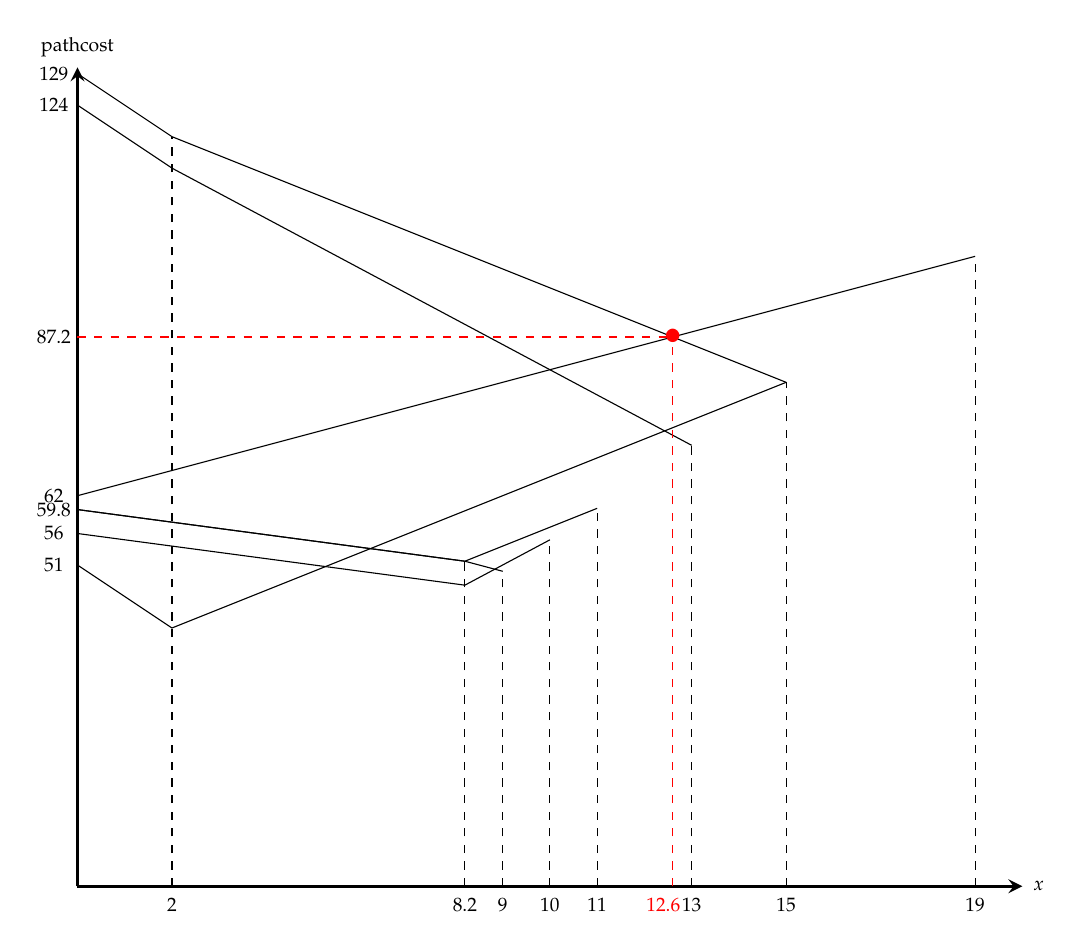
\begin{tikzpicture}[font=\scriptsize,>=stealth,yscale=0.08,xscale=0.6]
%		\draw [step=1cm,thick,dotted,draw=black!60] (0,0) grid (13,129);
		
		\draw [->, very thick] (0,0) -- (20,0) node[right] {$x$};
		\draw [->, very thick] (0,0) -- (0,130) node[above] {pathcost};
		
		\draw (0,56) -- (8.2,47.8) -- (10, 55);
		\draw (0,59.8) -- (8.2, 51.6) -- (9, 50);
		\draw (0,59.8) -- (8.2, 51.6) -- (11, 60);
		\draw (0,124) -- (2, 114) -- (13, 70);
		\draw (0,129) -- (2, 119) -- (15, 80);
		\draw (0,51) -- (2, 41) -- (15, 80);
		\draw (0,62) -- (19, 100);
		
		\node at (-.5, 56) {$56$};
		\node at (-.5, 59.8) {$59.8$};
		\node at (-.5, 124) {$124$};
		\node at (-.5, 129) {$129$};
		\node at (-.5, 51) {$51$};
		\node at (-.5, 62) {$62$};
		
		\draw [dashed] (2,0) -- (2, 119);
		\draw [dashed] (8.2,0) -- (8.2, 51.6);
		\draw [dashed] (9,0) -- (9, 50);
		\draw [dashed] (10,0) -- (10, 55);
		\draw [dashed] (11,0) -- (11, 60);
		\draw [dashed] (13,0) -- (13, 70);
		\draw [dashed] (15,0) -- (15, 80);
		\draw [dashed] (19,0) -- (19, 100);
		
		\node at (2,-3) {$2$};
		\node at (8.2,-3) {$8.2$};
		\node at (9,-3) {$9$};
		\node at (10,-3) {$10$};
		\node at (11,-3) {$11$};
		\node at (13,-3) {$13$};
		\node at (15,-3) {$15$};
		\node at (19,-3) {$19$};
		
		\draw [dashed, red] (0,87.2) -- (12.6,87.2);
		\draw [dashed, red] (12.6,0) -- (12.6,87.2);
		\node at (12.6, 87.2) {\large\color{red}$\bullet$};
		\node at (-.5,87.2) {$87.2$};
		\node at (12.4,-3) {\color{red}$12.6$};
		\end{tikzpicture}
	\end{center}
	\vskip -0.6cm
	\caption{Optimal shift at node 0}
	\label{fig:example_shift}
\end{figure}
Then the optimal shift of production to node 0 is 12.6, and the optimal solution is

\noindent\begin{tabular}{ccc c||}
	$T=1$ & $T=2$ & $T=3$ & path cost\\
		&		   & (1,\;0) & (68)\\
		& (6,\;0)  & (7,\;0) & (68)\\
		&		   & (2,\;0)& (68)\\
		&		   & (9,\;0.4)& (71.6)\\
(5,\;13.6) & (10,\;0) & (8,\;2.4)& ({\color{red}87.2})\\
		&		   & (2,\;2.4)& (72.8)\\
		&		   & (6,\;0)& ({\color{red}87.2})\\
		& (3,\;6.4)  & (2,\;0)& ({\color{red}87.2})\\
		&		   & (5,\;0)& ({\color{red}87.2})
\end{tabular}
\begin{minipage}{0.5\textwidth}
	\begin{itemize}
		\item If all curves are going downward, shift as much as possible.
		\item Only consider intersection of an upward segment and downward segment.
		\item Certain types of polylines cannot exist due to the optimality of subproblems.
		\item To get integral solutions, evaluate two adjacent integer points
		the optimal shift is a fraction.
	\end{itemize}
\end{minipage}

\section*{March 24th, 2015}
\subsection*{Dynamic programming formulation}
\subsubsection*{General formulation}
A general DP formulation of capacity planning problem is given as follows:
\begin{align*}
  & V_t(I_{t-1},\xi_t) =
  \min_{(x_t,y_t)\in \mathcal{F}_t(I_{t-1},\xi_t)} \left\{c_t(x_t,y_t)+\max_{\xi_{t+1}\in \mathcal{U}_{t+1}}V_{t+1}(I_t,\xi_{t+1})\right\} \quad \text{for } t=1,\dots, T,\\
  & V_{T+1}(I_T,\xi_{T+1}) = 0\quad \text{ for all } I_T\ge 0, \text{ and } \xi_{T+1},
\end{align*}
$V_t(I_{t-1},\xi_t)$ is the optimal cost from period $t$ to $T$ given the available capacity $I_{t-1}$ and uncertainty realization $\xi_t$.
$V_1(I_0, \xi_1)$ gives the optimal total cost.
In the above formulation, $\xi_t$ represents the uncertainty realization at period $t$, it contains generation cost and demand in our problem.
$I_t = \sum_{s=1}^{t}x_s$ is the total available capacity at the end of period $t$.
$c_t(x_t,y_t)$ represents the total of investment and generation cost at period $t$ with decision $(x_t,y_t)$. The corresponding feasible region is
\[\mathcal{F}_t(I_{t-1},\xi_t) = \left\{x_t\in \Z^{k_1}_+, y_t\in \R^{k_2}_+:
x_t - A_ty_t \ge -I_{t-1}, B_ty_t = d_t\right\}.\]

\subsubsection*{Scenario tree setting}
If we assume the uncertainty evolution is represented as a scenario tree, then a DP recursion
can be written as follows:
\begin{align*}
	& V_n(I_{a(n)},\xi_n) =
	\min_{(x_n,y_n)\in \mathcal{F}_n(I_{a(n)},\xi_n)} \left\{c_n(x_n,y_n)+
	\max_{m\in C_n}V_{m}(I_{n},\xi_{m})\right\} \quad \text{for } n\in \T,
\end{align*}
where $V_n(I_{a(n)},\xi_n)$ is the optimal cost on the subtree with root $n$ given the available capacity $I_{a(n)}$
and uncertainty realization $\xi_n$.
If node $n$ does not have any child node, i.e., $C_n=\emptyset$, the cost-to-go function is $0$.
$V_0(I_0,\xi_0)$ gives the optimal total cost.
Similarly, $\xi_n$ represents the uncertainty realization at node $n$.
$I_n = \sum_{m\in P[n]}x_m$ is the total available capacity at node $n$ (including investment at current node).
$c_n(x_n,y_n)$ represents the total of investment and generation cost at node $n$ with decision $(x_n,y_n)$.
The corresponding feasible region is
\[\mathcal{F}_n(I_{a(n)},\xi_n) = \left\{x_n\in \Z^{k_1}_+, y_n\in \R^{k_2}_+:
x_n - A_{n}y_n \ge -I_{a(n)}, B_ny_n = d_n\right\}.\]

\subsubsection*{Single-item problem}
Here we also present a DP formulation for the single-item problem, assuming that uncertainty evolution
is represented by a scenario tree.
\begin{align*}
& V_n(I_{a(n)},d_n) =
\min_{(x_n)\in \mathcal{F}_n(I_{a(n)},d_n)} \left\{c_n(x_n)+
\max_{m\in C_n}V_{m}(I_{n},d_{m})\right\} \quad \text{for } n\in \T,
\end{align*}
where
\[\mathcal{F}_n(I_{a(n)},d_n) = \left\{x_n\in \Z_+:
x_n \ge d_n-I_{a(n)}\right\}.\]

\section*{March 25, 2015}
\subsection*{Pareto robustly optimal v.s. Bellman optimal}
\citet{iancu2013pareto} define Pareto efficiency for robust linear problems.
In particular, they consider the following problem
\begin{align*}
\min \quad & \max_{c\in \mathcal{U}} c\cdot x\\
\subjectto \quad & x\in X = \{x: Ax\le b\}
\end{align*}
where $\mathcal{U} = \{c\in \R^n: Dc\le d\}$.
\begin{definition}
A solution $x$ is called \emph{Pareto robustly optimal} to the above problem if
(1) it is robustly optimal; (2) there does not exist an $\hat{x}\in X$ such that
(i) $c\cdot \hat{x} \le c\cdot x$ for all $c\in U$;
(ii) there exists $\hat{c}\in U$ such that $\hat{c}\cdot \hat{x} < \hat{c}\cdot x$. 
\end{definition}

We can define similar notion for problem \eqref{model:FAMS}.
\begin{definition}
	A solution $(\bx,\by)$ is called \emph{Pareto robustly optimal} to problem \eqref{model:FAMS} if
	\begin{enumerate}[topsep=0pt,noitemsep]
	\item it is robustly optimal;
	\item there does not exist an feasible $(\hat{\bx},\hat{\by})$ such that
	\begin{enumerate}[label=(\roman*)]
		\item $cost(\hat{\bx},\hat{\by},P) \le cost(\hat{\bx},\hat{\by},P)$ for all $P\in \cP$;
		\item there exist a path $\hat{P}\in \cP$ such that
		$cost(\hat{\bx},\hat{\by},P) < cost(\hat{\bx},\hat{\by},P)$
	\end{enumerate}
	\end{enumerate} 
\end{definition}

{\large \color{red} QUESTION: \color{blue}
	What is the connection between Pareto robustly optimal and Bellman Optimal?}

\section*{March 28, 2015}
\begin{proposition}~
	Bellman optimality and Pareto robustly optimality are not implied by each other.
\end{proposition}
\begin{proof}~
We consider the single-item problem (without $y$ variables).
	
\noindent\begin{tabular}{cc||}
	$T=1$ & $T=2$\\
	& (3,\;100)\\
(3,\;2)  &   \\
	& (5,\;4)
\end{tabular}
\begin{minipage}{0.8\textwidth}
	\begin{itemize}
		\item Both solutions $(2,(98,2))$ and $(4,(96,0))$ are Bellman optimal, but the only the second one is Pareto robustly optimal.
		In this case, Pareto robustly optimal solution is unique.
		\item Therefore, Bellman optimality $\notimplies$ Pareto robustly optimality.
	\end{itemize}
\end{minipage}

The following example serves as a counter-example of the reverse direction.

\noindent\begin{tabular}{ccc||}
	$T=1$ & $T=2$ & $T=3$\\
		& (4,\;2) & (3,\;100)\\
(3,\;1) & & \\
		& (5,\;3) & (10,\;10) \\
		& 	& (1,\;4)
\end{tabular}
$\quad$ $\bx^1:$
\begin{tabular}{ccc c||}
	$T=1$ & $T=2$ & $T=3$ & cost\\
	& (0) & (97) & 300\\
(3) & & & \\
	& (0) & (7) & 79 \\
	& 	& (1) & 10
\end{tabular}
$\quad$ $\bx^2:$
\begin{tabular}{ccc c||}
	$T=1$ & $T=2$ & $T=3$ & cost\\
	& (0) & (97) & 300\\
(3) & & & \\
	& (7) & (0) & 44 \\
	& 	& (0) & 44
\end{tabular}
It is easy to check that $\bx^1$ is Pareto robustly optimal.
Indeed, the last path has the lowest possible cost.
However, $\bx^1$ is not Bellman optimal, instead, $\bx^2$ is.
Therefore, Pareto robustly optimality does not imply Bellman optimality.
\end{proof}

Another interesting observation from the above example is that,
even though $\bx^2$ is Bellman optimal, it is not Pareto robustly optimal.
Consider solution $\bx^3$:
\begin{tabular}{ccc c}
	$T=1$ & $T=2$ & $T=3$ & path cost\\
	& (0) & (90) & 300\\
(10) & & & \\
	& (0) & (0) & 30 \\
	& 	& (0) & 30
\end{tabular}.
This solution is Bellman {\bf AND} Pareto robust optimal.

{\color{blue} Thus, it seems that the ``best" solution (policy) one should look for is both Bellman optimal and Pareto robustly optimal.
The first optimality guarantees the policy to be implementable without resolving the problem as uncertainty reveals.
The second optimality ensures that there is no other policy such that it decreases the cost for some scenario without increasing the costs for any others.}

The figure below illustrates the relations between different optimality
standards in multi-stage robust optimization problems, {\bf assuming the uncertainty evolution is represented as a scenario tree}.
\begin{figure}[htb!]
\begin{center}
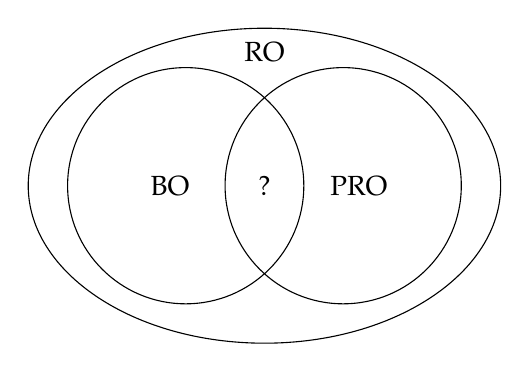
\begin{tikzpicture}
\draw (0,0) ellipse (3cm and 2cm);
\draw (1,0) circle (1.5cm);
\draw (-1,0) circle (1.5cm);
\node at (0,1.7) {RO};
\node at (-1.2,0) {BO};
\node at (1.2,0) {PRO};
\node at (0,0) {?};
\end{tikzpicture}
\caption{Different optimality standards in multi-stage robust optimization}
\label{fig:optimality-relation}
\end{center}
\end{figure}

For general multi-stage robust optimization problems, {\color{red}we may define} RO to be the set that contains
all optimal solutions to the formulation where the decision variables correspond to policies, i.e.,
\begin{subequations}\label{formulation:policy}
\begin{align}
\min_{x_1, x_2(\cdot), \ldots, x_T(\cdot)}\quad & \max_{(\xi_2,\ldots,\xi_T)\in \mcal{D}} [f_1(x_1)+f_2(x_2,\xi_2)+ \cdots + f_{T}(x_T,\xi_T)]\\
\subjectto \qquad\quad & x_1\in \mcal{X}_1,\quad x_t\in \mcal{X}_t(x_{t-1},\xi_{t-1}), \quad t=2,\ldots, T.
\end{align}
\end{subequations}
See \citet{shapiro2011dynamic} for details of notation.

By definition, the set BO (Bellman optimality) contains all optimal 
solutions to the DP formulation.
\begin{subequations}\label{formulation:DP}
\begin{align}
& \min_{x_1\in \mcal{X}_1}\quad \left\{f_1(x_1) + \max_{\xi_{[2]}\in \mcal{D}_2} Q_2(x_2, \xi_{[2]})\right\}\\
& Q_{t}(x_{t-1},\xi_{[t]}) = \min_{x_t\in \mcal{X}_{t}(x_{t-1},\xi_t)}\left\{ f_t(x_t,\xi_t) + \max_{\xi_{[t+1]}\in \mcal{D}_{t+1}} \left\{Q_{t+1}(x_t, \xi_{[t+1]}) \right\} \right\}, \quad \forall t=2,\ldots, T,
\end{align}
\end{subequations}
with $Q_{T+1}(\cdot,\cdot) = 0$ by definition,
and $\mcal{D}_t$ is the projection of $\mcal{D}$ onto $\R^{d_2}\times\cdot\times \R^{d_t}$.

{\color{blue}
	\citet{shapiro2011dynamic} states the condition under which Model \eqref{formulation:policy} and \eqref{formulation:DP} share the same optimal objective function value, and each optimal solution to \eqref{formulation:DP} is also optimal to \eqref{formulation:policy}.
}

To introduce Pareto robustly optimality in this setting, we use the following
equivalent epigraph formulation.
\begin{subequations}\label{formulation:epigraph}
	\begin{align}
	\min_{z, x_1, x_2(\cdot), \ldots, x_T(\cdot)}\quad & z\\
	\subjectto \qquad\quad & z \ge \sum_{t=1}^{T}f_t(x_t,\xi_t),\quad \forall~\xi_{[T]}\in \mcal{D},\\
	& x_1\in \mcal{X}_1,\quad x_t\in \mcal{X}_t(x_{t-1},\xi_{t-1}), \quad t=2,\ldots, T.
	\end{align}
\end{subequations}
Let $\mcal{C}$ be the set of constraints.
For policy $\bx$ and uncertainty realization $\xi_{[T]}$, we associate a ``{\it slack}" $s_j(\bx,\xi_{[T]})$, together with a ``slack value" $v_j$,
with each constraint.
Then an PRO policy can be defined as follows:
\begin{definition}
	A policy $\{x_1, x_2(\cdot), \ldots, x_T(\cdot)\}$ is called
	\emph{Pareto robustly optimal} to problem \eqref{formulation:epigraph} if
	there does not exist an robustly optimal policy $\{\hat{x}_1, \hat{x}_2(\cdot), \ldots, \hat{x}_T(\cdot)\}$ such that
	\begin{enumerate}[topsep=0pt,noitemsep,label=(\roman*)]
		\item $\sum_{j\in \mcal{C}}v_js_j(\hat{\bx},\xi_{[T]}) \ge \sum_{j\in \mcal{C}}v_js_j(\bx,\xi_{[T]})$
		for all $\xi_{[T]}\in \mcal{D}$;
		\item there exists some scenario $\hat{\xi}_{[T]}\in \mcal{D}$ such that
		$\sum_{j\in \mcal{C}}v_js_j(\hat{\bx},\hat{\xi}_{[T]}) \ge \sum_{j\in \mcal{C}}v_js_j(\bx,\hat{\xi}_{[T]})$.
	\end{enumerate}
\end{definition}

\newpage
\section*{April 10, 2015}
Let us consider the following distributionally robust optimization problem
\begin{equation}\label{problem:DROP}
\min_{x\in \mcal{X}}~\max_{P\in \mcal{P}}~\mathbb{E}_{P}[f(x,\xi)],\tag{DROP}
\end{equation}
where $\mcal{X}\subset \R^n$ is a convex, bounded feasible set, $\mcal{P}$ is a set of distributions of $\xi$. $f: \R^n\times \R^m\to \R$ is the cost function and
is convex in $x$; $\xi$ is a random vector in $\R^m$.
We would like to address the Pareto distributionally robust optimality defined as follows.
\begin{definition}[Pareto Distributionally Robust Optimal (PDRO)]
	Let $x^*$ be an optimal solution to Problem \eqref{problem:DROP}.
	It is \emph{Pareto distributionally robust optimal} if there does not exist
	$\hat{x}\in \mcal{X}$ such that the following
	conditions are satisfied:
	\begin{enumerate}[topsep=0pt,noitemsep,label=(\roman*)]
		\item $\mathbb{E}_P[f(\hat{x},\xi)] \le \mathbb{E}_P[f(x^*,\xi)]$ for all $P\in \mcal{P}$;
		\item There exists some $\hat{P}\in\mcal{P}$ such that
		$\mathbb{E}_{\hat{P}}[f(\hat{x},\xi)] < \mathbb{E}_{\hat{P}}[f(x^*,\xi)]$.
	\end{enumerate}
\end{definition}

{\color{blue}
\begin{note}
In problem \eqref{problem:DROP}, if we use the distribution set $\mcal{P}$ where
each $P\in \mcal{P}$ is a distribution that puts all weight on one point $\xi\in \Xi$, the model corresponds to the robust model
\[\min_{x\in \mcal{X}}~\max_{i}~f(x,\xi^i).\]
\end{note}
}

\subsection*{Does PDRO solution always exist?}
No proof nor counter-example yet... 


\subsection*{Finite support for $\boldsymbol\xi$}
Suppose $\xi$ has finite support $\{\xi^1,\dots, \xi^k\}$. Then $\mcal{P}$ is
a subset of probability simplex in $\R^k$. Thus a realization $P\in \mcal{P}$ is
just a vector $p\in \R^k_+$ that satisfies $e\tr p = 1$. For simplicity, we assume that $\mcal{P}$ is a polytope, i.e.,
$\mcal{P} = \{p\in \R^k_+: Dp\le d\}$, where $Dp\le d$ contains $e\tr p = 1$.  
We consider different cases for the cost function $f$ and feasible region $\mcal{X}$.

\subsubsection*{A1: $\mcal{X}$ is polyhedron, $f(\cdot,\cdot)$ is linear}
In this case, our problem becomes exactly the same as the one addressed in
\citet{iancu2013pareto}, in which the adversary uncertainty set is defined as
$U = \{u=\Xi p: p\in \mcal{P}\}$, where $\Xi = \{\xi^1,\dots, \xi^k\}$.

\subsubsection*{A2: $f(\cdot,\cdot)$ is convex in $x$}
We further assume that for each $x\in \mcal{X}$ and $\xi^i$, $i=1,\dots, k$,
$f(x,\xi)<\infty$. Under such assumptions, the problem is
\begin{equation}\label{case2}
\min_{x\in \mcal{X}}~\max_{p\in \mcal{P}}~p\tr f(x).
\end{equation}
where $f(x) = (f(x,\xi^1),\dots, f(x,\xi^k))\tr$.
Notice that an optimal solution always exists and the inner maximization problem yields a convex function in $x$.
Let $X^{\text{DRO}}$ be the set of optimal solutions to \eqref{case2}.
Taking the dual of inner maximization problem yields a convex optimization problem.
Let $z^{\text{DRO}}$ be the optimal value of \eqref{case2}. Then the set $X^{\text{DRO}}$ can be represented as the following convex set.
\[X^{\text{DRO}} = \{x\in \mcal{X}: \exists \beta\ge 0 \text{ such that } D\tr\beta\ge f(x), d\tr\beta \le x^{\text{DRO}}\}.\]

We now have two questions to answer, i.e.,
\begin{enumerate}[topsep=0pt,noitemsep,label=(\arabic*)]
	\item How to verify if a given DRO solution is PDRO?
	\item How to find one PDRO solution if there always exists one?
\end{enumerate}

\paragraph{How to verify if a given DRO solution is PDRO?}
Suppose given a DRO solution $x$, one would like to know if $x$ is also PDRO or not.
Consider any point $\bar{p}\in \text{ri}(\cP)$, we solve the following convex program:
\begin{subequations}\label{verify_problem}
\begin{align}
\min_{y,z}\quad & \bar{p}\tr z\\
\subjectto \quad & f(x+y)\le f(x) + z\\
& z\in \cP^o\\
&x+y\in \mcal{X},
\end{align}
\end{subequations}
where $P^o= \{z\in\R^k: p\tr z\le 0, \forall p\in \cP\}$ is the polor cone of set $\cP$.
It is easy to verify that $(0,0)$ is feasible to \eqref{verify_problem}.
Therefore, the optimal value $v^*(x,\bar{p})$ is non-positive.
\begin{itemize}[topsep=0pt,noitemsep]
	\item {\color{red} Suppose $v^*(x,\bar{p}) = 0$. We claim that $x$ is PDRO.}
	Suppose not, there exists some $\hat{x}$ that Pareto distributionally dominates $x$, i.e.,
	(i) $p\tr f(\hat{x}) \le p\tr f(x)$ for all $p\in \cP$;
	(ii) there exists some $\hat{p}\in \cP$ such that $\hat{p}\tr f(\hat{x}) < \hat{p}\tr f(x)$. Without loss of generality, we assume $\hat{p}$ to be a boundary point optimal solution to the problem $\min_{p\in \cP}p\tr (f(\hat{x}) - f(x))$.
	Note that $(\hat{x}-x, f(\hat{x})-f(x))$ is feasible to \eqref{verify_problem}.
	Next we show that $\bar{p}(f(\hat{x})-f(x))<0$.
	In fact, $\bar{p}$ can be represented by a strictly convex combination of extreme
	points of $\cP$ \citep[see][]{rockafellar1970convex}, i.e.,
	there exists $\lambda\in \R^{|\text{ext}(\cP)|}_{++}$ such that
	$\bar{p} = \lambda_ip^i$.
	It follows that
	\[\bar{p}\tr(f(\hat{x})-f(x)) = \lambda_i\hat{p}\tr (f(\hat{x})-f(x)) +
	\sum_{i:p_i\neq \hat{p}}\lambda_i {p^i}\tr (f(\hat{x})-f(x)) < 0,\]
	contradicts to the fact that  $v^*(x,\bar{p}) = 0$.
	
	\item {\color{red} Suppose $v^*(x,\bar{p}) < 0$.}
	Let $(y^*,z^*)$ be the optimal solution to \eqref{verify_problem},
	and denote $\tilde{x} = x+y^*$.
	{\color{red}We claim that $\tilde{x}$ is PDRO.}
	It is easy to verify that $\tilde{x}$ Pareto distributionally dominates $x$.
	Next we claim that solving problem \eqref{verify_problem} with $x$ substituted
	with $\tilde{x}$ yield optimal value 0, hence $\tilde{x}$ is PDRO.
	Suppose not, let $(\tilde{y},\tilde{z})$ be the optimal solution with
	$\bar{p}\tr \tilde{z} <0$.
	Since $f(x+y^*+\tilde{y}) = f(\tilde{x}+\tilde{y}) \le f(\tilde{x}) + \tilde{z} \le f(x)+z^*+\tilde{z}$,
	$z^*+\tilde{z}\in \cP^o$, and $x+y^*+\tilde{y}\in \mcal{X}$,
	we know that $(y^*+\tilde{y},z^*+\tilde{z})$ is feasible to \eqref{verify_problem}. However, this solution yields a better objective function
	value, i.e., $\bar{p}\tr (z^*+\tilde{z}) < \bar{p}\tr z^*$, contradicting to
	the optimality of $(y^*,z^*)$.
\end{itemize}
\paragraph{How to find a PDRO solution if there always exists one?}
The above argument implies that under such settings, a PDRO solution always exist.
It follows that we can can a PDRO solution by solving
$\min_{x\in X^{\text{RO}}} \bar{p}\tr f(x)$ for any given $\bar{p}\in \text{ri}(\cP)$, which is a convex program.

{\color{blue}In fact, we can rewrite problem \eqref{case2} as follows
\begin{equation}\label{case2_tf}
\min_{z\in \mcal{Z}}~\max_{q\in \mcal{Q}}~q\tr z
\end{equation}
where $\mcal{Z} = \{z=(x,t)\in \R^{n+k}:f(x)\le t, x\in \mcal{X}\}$,
and $\mcal{Q} = \{q=(0,p)\in \R^{n+k}: p\in \mcal{P}\}$.
Now $Z$ is convex (since we assume $f(x)<\infty$ we can add some upper bound on $t$
so that $Z$ becomes compact). $\mcal{Q}$ is a polyhedron in higher dimension.
Theorem 1, Corollary 1 \& 2, Proposition 1 \& 2 in \citet{iancu2013pareto} are all valid under such generalization.

An immediate next step is to generalize the set $\cP$.
}

\section*{April 23, 2015}
\subsection*{Non-convexity of PRO Set}
\citet{iancu2013pareto} gives an example which shows that the PRO set is not convex in general. 

%\section*{April 12, 2015 --- A multi-level approach}
%Suppose we are solving the following problem
%\begin{equation}\label{level1}
%\min_{x\in \mcal{X}}~\max_{i}~f(x,\xi^i).
%\end{equation}
%An optimal solution achieves the worst-case cost $v_1^*$.
%The costs along some non-worst-case paths, however, can still be reduced.
%We continue to solve the following problem, which minimizes the largest sum of
%two scenario costs.
%\begin{subequations}\label{level1}
%	\begin{align*}
%	\min_{x} \quad & \max_{z\in \{0,1\}^k:e\tr z = 2}~z\tr f(x)\\
%	\subjectto \quad & \max_{i}f(x,\xi^i) \le v_1^*\\
%	& x\in \mcal{X}
%	\end{align*}
%\end{subequations}


%%% References
\newpage
\bibliographystyle{plainnat}
\bibliography{bibliography}

\end{document}
 






